
%========= File containing the main LaTex document ========%
%                                                         
%
%
%==========================================================%

\documentclass[pfe]{./tpl/isipfe}
\graphicspath{{./img/}}

%\usepackage{hyperref}
\usepackage{array}
\usepackage{lipsum}
\usepackage{multirow}
\usepackage{longtable}

%=========== File containing some new commands ============%
%                                                          %
%==========================================================%

\newenvironment{changemargin}[2]{%
\begin{list}{}{%
\setlength{\leftmargin}{#1}%
\setlength{\rightmargin}{#2}%
}%
\item[]}
{\end{list}}

\makeatletter

%================= front cover variables =================%

\newcommand{\secondAuthor}[1]{\gdef\@secondAuthor{#1}}%
\newcommand{\@secondAuthor}{\@latex@warning@no@line{No \noexpand\secondAuthor given}}

\newcommand{\diplomaName}[1]{\gdef\@diplomaName{#1}}%
\newcommand{\@diplomaName}{\@latex@warning@no@line{No \noexpand\diplomaName given}}

\newcommand{\speciality}[1]{\gdef\@speciality{#1}}%
\newcommand{\@speciality}{\@latex@warning@no@line{No \noexpand\speciality given}}

\newcommand{\proFramerName}[1]{\gdef\@proFramerName{#1}}%
\newcommand{\@proFramerName}{\@latex@warning@no@line{No \noexpand\proFramerName given}}

\newcommand{\proFramerSpeciality}[1]{\gdef\@proFramerSpeciality{#1}}%
\newcommand{\@proFramerSpeciality}{\@latex@warning@no@line{No \noexpand\proFramerSpeciality given}}

\newcommand{\academicFramerName}[1]{\gdef\@academicFramerName{#1}}%
\newcommand{\@academicFramerName}{\@latex@warning@no@line{No \noexpand\academicFramerName given}}

\newcommand{\academicFramerSpeciality}[1]{\gdef\@academicFramerSpeciality{#1}}%
\newcommand{\@academicFramerSpeciality}{\@latex@warning@no@line{No \noexpand\academicFramerSpeciality given}}

\newcommand{\collegeYear}[1]{\gdef\@collegeYear{#1}}%
\newcommand{\@collegeYear}{\@latex@warning@no@line{No \noexpand\collegeYear given}}

\newcommand{\companyName}[1]{\gdef\@companyName{#1}}%
\newcommand{\@companyName}{\@latex@warning@no@line{No \noexpand\companyName given}}

%================== Signatures variables ==================%

\newcommand{\proSignSentence}[1]{\gdef\@proSignSentence{#1}}%
\newcommand{\@proSignSentence}{\@latex@warning@no@line{No \noexpand\proSignSentence given}}

\newcommand{\academicSignSentence}[1]{\gdef\@academicSignSentence{#1}}%
\newcommand{\@academicSignSentence}{\@latex@warning@no@line{No \noexpand\academicSignSentence given}}

%================== Backcover variables ==================%

\newcommand{\arabicAbstract}[1]{\gdef\@arabicAbstract{#1}}%
\newcommand{\@arabicAbstract}{\@latex@warning@no@line{No \noexpand\arabicAbstract given}}

\newcommand{\arabicAbstractKeywords}[1]{\gdef\@arabicAbstractKeywords{#1}}%
\newcommand{\@arabicAbstractKeywords}{\@latex@warning@no@line{No \noexpand\arabicAbstractKeywords given}}

\newcommand{\frenchAbstract}[1]{\gdef\@frenchAbstract{#1}}%
\newcommand{\@frenchAbstract}{\@latex@warning@no@line{No \noexpand\frenchAbstract given}}

\newcommand{\frenchAbstractKeywords}[1]{\gdef\@frenchAbstractKeywords{#1}}%
\newcommand{\@frenchAbstractKeywords}{\@latex@warning@no@line{No \noexpand\frenchAbstractKeywords given}}

\newcommand{\englishAbstract}[1]{\gdef\@englishAbstract{#1}}%
\newcommand{\@englishAbstract}{\@latex@warning@no@line{No \noexpand\englishAbstract given}}

\newcommand{\englishAbstractKeywords}[1]{\gdef\@englishAbstractKeywords{#1}}%
\newcommand{\@englishAbstractKeywords}{\@latex@warning@no@line{No \noexpand\englishAbstractKeywords given}}

\newcommand{\companyEmail}[1]{\gdef\@companyEmail{#1}}%
\newcommand{\@companyEmail}{\@latex@warning@no@line{No \noexpand\companyEmail given}}

\newcommand{\companyTel}[1]{\gdef\@companyTel{#1}}%
\newcommand{\@companyTel}{\@latex@warning@no@line{No \noexpand\companyTel given}}

\newcommand{\companyFax}[1]{\gdef\@companyFax{#1}}%
\newcommand{\@companyFax}{\@latex@warning@no@line{No \noexpand\companyFax given}}

\newcommand{\companyAddressFR}[1]{\gdef\@companyAddressFR{#1}}%
\newcommand{\@companyAddressFR}{\@latex@warning@no@line{No \noexpand\companyAddressFR given}}

\newcommand{\companyAddressAR}[1]{\gdef\@companyAddressAR{#1}}%
\newcommand{\@companyAddressAR}{\@latex@warning@no@line{No \noexpand\companyAddressAR given}}

%============= cmd for inserting blank page =============%
\newcommand\blankpage{%
    \null
    \thispagestyle{empty}%
    \addtocounter{page}{-1}%
    \newpage}

%================ document main language ================%
%\selectlanguage{english}
\selectlanguage{french}

%================== required packages ===================%

\usepackage{tcolorbox}
\usepackage{afterpage}
\usepackage{array,longtable,multirow}% http://ctan.org/pkg/{array,longtable,multirow}
\usepackage{pifont}

\usepackage{pdflscape}
\usepackage{rotating}
\usepackage{wrapfig}

\begin{document}
    
%=== File containing Global Configuration of the report ===%
%                                                          %
% Copyright (C) ISI - All Rights Reserved                  %
% Proprietary                                              %
% Written by Med Hossam <med.hossam@gmail.com>, April 2016 %
%                                                          %
% @author: HEDHILI Med Houssemeddine                       %
% @linkedin: http://tn.linkedin.com/in/medhossam           %
%==========================================================%

%=========== You MUST type your information here ==========%
% global_config.tex file is designed to configure your     %
% cover pages (main, back and black covers)                %
%==========================================================%

%============= Config new columns type ==============%
\newcolumntype{L}{>{\raggedright\arraybackslash}}
\newcolumntype{R}{>{\raggedleft\arraybackslash}}
\newcolumntype{C}{>{\centering\arraybackslash}}
%==================================================%

%========= Config the cover section ==========%

\title{Mise en place d'une application de gestion des agences et des utilisateurs dans le domaine Assurtech }

\author{Haithem FRAD}
%%% if necessary
% Set isBinomal to true and type second author name
%\setboolean{isBinomal}{true}
%\secondAuthor{Prénom NOM}

\diplomaName{Diplôme National d'Ingénieur en Informatique}
\speciality{Ingénierie des Systèmes Intelligents  }
%\speciality{Génie des Télécommunications et Réseaux}
%\speciality{Génie Informatique des Systèmes Industriels}

%% Encadrant professionnel
\proFramerName{Hamdi Bousleh}
\proFramerSpeciality{Manager}

%% Encadrant académique
\academicFramerName{}
\academicFramerSpeciality{}

%% Entreprise d'accueil
\companyName{Dqlick}

%% Année universitaire
\collegeYear{2019 - 2020}

%%%%%% Signatures section %%%%%%

% You can simply remove theses sentences by typing an empty string
% \proSignSentence{}

\proSignSentence{}

\academicSignSentence{}

%%% AR
\arabicAbstract{}

\arabicAbstractKeywords{}

%% To use latin characters inside the arabic text
% just put them inside the command \textLR{}
%%%%

%%% FR
\frenchAbstract{}

\frenchAbstractKeywords{}

%%% EN
\englishAbstract{}

\englishAbstractKeywords{}

%% if you want to get rid of the company address just set the boolean variable to false
% PS : it's optional
\setboolean{wantToTypeCompanyAddress}{true}

\companyEmail{contact@dqlick.com}
\companyTel{71 965 425}
\companyAddressFR{immeuble ADONIS, rue du Lac d’Annecy
Les Berges du Lac 1053}
    
    \frontmatter
        
%===== File containing the main cover of the document =====%
%                                                          %
% Copyright (C) ISI - All Rights Reserved                  %
%==========================================================%

%== It's advised to not modify the content of this file ===%
% To set your information, go to global_config.tex file    %
%==========================================================%

\thispagestyle{cover}%
\newgeometry{bottom=25mm,left=20mm,top=15mm,right=20mm}
\hspace{-47pt}
\begin{minipage}[l]{0.2\columnwidth}
\vspace{6mm}

\includegraphics[width=1\columnwidth]{images/logos/logo_enicar.jpg}\\
\end{minipage}
\hfill
\begin{minipage}[l]{0.6\columnwidth}
\centering
\footnotesize
\textbf{{République Tunisienne}}\\
\vspace{1.5mm}
\textbf{{Ministère de l'Enseignement Supérieur\\
et de la Recherche Scientifique}}\\
\vspace{1.5mm}
\textbf{{Université de Carthage}}\\
\vspace{1.5mm}
\textbf{{École Nationale d'Ingénieurs de Carthage}}
\end{minipage}
\hfill
\begin{minipage}[l]{0.02\columnwidth}
\end{minipage}
\hfill
\begin{minipage}[l]{0.18\columnwidth}
\vspace{6mm}

\includegraphics[width=1\columnwidth]{images/logos/logo_ucar.png}\\
\end{minipage}
\vskip1.5cm

\begin{center}
{\LARGE{\textbf{\textsc{Rapport de Stage Ingénieur}}}}\\
\vskip0.5cm
\large

{\textbf{Présenté en vue de l'obtention du}}\\
\vskip2mm
{\textbf{\@diplomaName}}\\
{\textbf{Spécialité : \@speciality}}\\
{}
\end{center}

\begin{center}
\textrm{Par}\\
\vskip0.3cm
{\ifthenelse{\boolean{isBinomal}}
    {% IF TRUE
        \begin{center}
            \large\textbf{\@author}~~~~~ et ~~~~~
            \large\textbf{\@secondAuthor}
        \end{center}
    }
    {\Large\textbf{\@author}}% FALSE
}
\vskip12mm

\definecolor{isiBlue}{RGB}{31, 78, 121}

\begin{changemargin}{-9mm}{0cm}
\begin{minipage}[l]{1.1\columnwidth}
\begin{tcolorbox}[colframe=isiBlue,colback=white,boxrule=0pt,toprule=3pt,bottomrule=3pt,arc=0pt,top=0mm,right=0mm,left=0mm,bottom=0mm,boxsep=0.5mm]{
    \begin{tcolorbox}[colframe=isiBlue,colback=white, boxrule=0pt,toprule=1pt,bottomrule=1pt,arc=0pt,enlarge bottom by=-0.9mm, auto outer arc]
        \centering
        {\huge\textbf{\@title}}
    \end{tcolorbox}
}
\end{tcolorbox}
\end{minipage}
\end{changemargin}

\end{center}
\vskip8mm%

\begin{center}
\large
\begin{minipage}[c]{0.28\columnwidth}
Encadrant professionnel:\\
%Encadrant académique:
\end{minipage}
\hfill
\begin{minipage}[c]{0.42\columnwidth}
\textbf{\@proFramerName}\\
%\textbf{\@academicFramerName}
\end{minipage}
\hfill
\begin{minipage}[c]{0.26\columnwidth}
\@proFramerSpeciality\\
\@academicFramerSpeciality
\end{minipage}
\end{center}
\vskip16mm

\begin{center}
\large
Réalisé au sein de \@companyName\\
\vskip0.05cm
\begin{figure}[h]
\centering
{{\fboxrule=1pt\fbox{
\includegraphics[width=0.2\columnwidth]{images/logo_Dqlick.png}}}}
\end{figure}
\end{center}


\begin{figure}[h]
\centering

\includegraphics[width=0.6\columnwidth]{images/logo_Dqlick.png}
\end{figure}

\end{center}
\afterpage{\blankpage}
        
%===== File containing the black cover of the document ====%
%                                                          %
%== It's advised to not modify the content of this file ===%
% To set your information, go to global_config.tex file    %
%==========================================================%

\thispagestyle{cover}%
\hspace{-47pt}
\begin{minipage}[l]{0.2\columnwidth}
\vspace{6mm}
\includegraphics[width=1.1\columnwidth]{Logo_ISI_Black}\\
\end{minipage}
\hfill
\begin{minipage}[l]{0.6\columnwidth}
\centering
\footnotesize
\textbf{{République Tunisienne}}\\
\vspace{1.5mm}
\textbf{{Ministère de l'Enseignement Supérieur\\
et de la Recherche Scientifique}}\\
\vspace{1.5mm}
\textbf{{Université de Tunis El Manar}}\\
\vspace{1.5mm}
\textbf{{Institut Supérieur d'Informatique d’El Manar}}
\end{minipage}
\hfill
\begin{minipage}[l]{0.02\columnwidth}
\end{minipage}
\hfill
\begin{minipage}[l]{0.18\columnwidth}
\vspace{6mm}
\includegraphics[width=0.9\columnwidth]{Logo_UTM_Black}\\
\end{minipage}
\vskip1.5cm

\begin{center}
{\LARGE{\textbf{\textsc{Rapport de Stage Ingénieur}}}}\\
\vskip0.5cm
\large

{\textbf{Présenté en vue de l'obtention du}}\\
\vskip2mm
{\textbf{\@diplomaName}}\\
{\textbf{Spécialité : \@speciality}}\\
{}
\end{center}

\begin{center}
\textrm{Par}\\
\vskip0.3cm
{\ifthenelse{\boolean{isBinomal}}
    {% IF TRUE
        \begin{center}
            \large\textbf{\@author}~~~~~ et ~~~~~
            \large\textbf{\@secondAuthor}
        \end{center}
    }
    {\Large\textbf{\@author}}% FALSE
}
\vskip12mm

\begin{changemargin}{-9mm}{0cm}
\begin{minipage}[l]{1.1\columnwidth}
\begin{tcolorbox}[colback=white,boxrule=0pt,toprule=3pt,bottomrule=3pt,arc=0pt,top=0mm,right=0mm,left=0mm,bottom=0mm,boxsep=0.5mm]{
    \begin{tcolorbox}[colback=white, boxrule=0pt,toprule=1pt,bottomrule=1pt,arc=0pt,enlarge bottom by=-0.9mm, auto outer arc]
        \centering
        {\huge\textbf{\@title}}
    \end{tcolorbox}
}
\end{tcolorbox}
\end{minipage}
\end{changemargin}

\end{center}
\vskip8mm%

\begin{center}
\large
\begin{minipage}[c]{0.28\columnwidth}
Encadrant professionnel:\\
\end{minipage}
\hfill
\begin{minipage}[c]{0.42\columnwidth}
\textbf{\@proFramerName}\\
\textbf{\@academicFramerName}
\end{minipage}
\hfill
\begin{minipage}[c]{0.26\columnwidth}
\@proFramerSpeciality\\
\@academicFramerSpeciality
\end{minipage}
\end{center}
\vskip16mm

\begin{center}
\large
Réalisé au sein de \@companyName\\
\vskip0.2cm
\begin{figure}[h]
\centering
{{\fboxrule=1pt\fbox{
\includegraphics[width=0.2\columnwidth]{images/logo_Dqlick.png}}}}
\end{figure}
\end{center}

\restoregeometry
        \thispagestyle{empty}

\begin{center}
    \begin{minipage}[l]{1\columnwidth}
        \begin{tcolorbox}[colback=white,boxrule=2pt,arc=10pt,height=120mm]{
            \vspace{2cm}
            \vspace{1mm}
            \begin{center}
                \Large
                Encadrant professionnel
                
                \textbf{\@proFramerName}
            \end{center}
            \vspace{5mm}
            \hspace{0.60\columnwidth}\textbf{\large Signature et cachet}
        }
        \end{tcolorbox}
    \end{minipage}
    
    \vspace{2cm}
    

\end{center}
        
        \setcounter{page}{1}
        \chapter*{\Huge Dédicaces}

\vspace{5cm}
\textit{\Large Je commence par rendre grâce à Dieu et sa volonté pour la patience, le courage et la compétence qu’il m’a donné pour   réaliser ce travail.}
















\begingroup
    \large \raggedright 
    \vspace{6mm}
    

    
    \vspace{6mm}
   
\endgroup

\vspace{10cm}
\begin{flushright}
    \LARGE \@author
\end{flushright}
        \thispagestyle{frontmatter}
        \chapter*{\huge \vspace{2cm} Remerciements}
\textit{\Large
\vspace{0.5cm}Durant  ce travail, je remercie chаleureusement mon encadrant \vspace{0.5cm}Monsieur Hamdi Bouslah, qui a fait preuve d'une grande patience      \vspace{0.5cm}en répondant à toutes mes questions et en essayant d’élargir mes \vspace{0.5cm}connaissances. A ce titre, j’exprime ma gratitude à toute l’équipe de \vspace{0.5cm}la société Dqlick pour leur accueil et leur esprit d’équipe.
\vspace{0.5cm}J'aimerais aussi  adresser mes remerciements les plus sincères et \vspace{0.5cm}exprimer ma reconnaissance à toutes les personnes qui auront contribué \vspace{0.5cm}de près ou de loin à l’élaboration de ce projet.}
\begin{center}
\it \Large
   
\end{center}
        \thispagestyle{frontmatter}
        
        \setcounter{secnumdepth}{3}
        \setcounter{tocdepth}{2}
        \dominitoc
        \tableofcontents
        \adjustmtc
        \thispagestyle{frontmatter}
        
        \listoffigures
        \thispagestyle{frontmatter}
        \listoftables
        \thispagestyle{frontmatter}
        

    
    \mainmatter
        \chapter*{Introduction générale}
\addcontentsline{toc}{chapter}{Introduction générale} % to include the introduction to the table of content
\markboth{Introduction générale}{} %To redefine the section page head

{\vspace{1cm \large Le marché de l'assurance est en pleine mutation : Nouvelles attentes de l’assuré, plus digital, plus volatil et mieux informé,  durcissement du cadre réglementaire, concurrence de plus en plus forte. Pour rester compétitifs, les assureurs doivent sans cesse se réinventer, innover et simplifier leur offre, leur distribution et leur relation assuré.\\
Dans ce contexte, optimiser les processus de gestion de l’assurance et accélérer la distribution directe et indirecte  sont deux chantiers de transformation digitale à prioriser car ils donneront aux assureurs un temps d'avance sur le marché, sur leurs concurrents et sur leurs objectifs de performance.\\
c'est pour cela les assurtech sont apparus. En effet, ce sont des entreprises exerçant dans le secteur de l’assurance. Elles s’appuient sur les nouvelles technologies pour introduire des innovations qui conduisent inéluctablement à l’éclosion de nouveaux modèles économiques, de nouveaux processus, de nouveaux produits.
Ces transformations profondes ont la capacité de modifier les comportements de tous les acteurs du marché : assurés, intermédiaires d’assurance, assureurs, réassureurs.
Les solutions offertes par les assurtech sont plus nombreuses en assurance non vie. Les investissements réalisés y sont plus importants du fait de la forte présence de la télémétrie dans les assurances automobile, santé et habitation.\\
Les améliorations qu’elles tentent d’apporter dans ce secteur visent à développer et enrichir les services offerts aux assurés tout en réduisant les coûts.}}
        \clearpage
        
        \chapter{Cadre général du projet}
\section*{Introduction}
Dans ce chapitre, nous allons présenter le cadre général du projet. Tout d'abord, nous présentons l'organisme d'accueil "Dqlick". Puis nous passons à la description du contexte de notre travail. Ensuite, nous expliquons la méthodologie du travail que nous avons adopté.

% Une section

% Exemple d'une section qui porte une référence à une bibliographie
% NB: il faut bien suivre le syntaxe pour ne pas tomber dans le cas où il y a une référence dans la table des matières.
\section {Présentation de l’organisme d’accueil Dqlick}

Dqlick est un éditeur de logiciels en marque blanche, permettant de couvrir tout le périmètre des activités des assurances, de gérer l’ensemble des contrats, d’innover en terme de gamme de produits tout en réduisant les contraintes de délais et de coûts. Dqlick s'adapte à tous les métiers avec un catalogue riche en fonctionnalités.
 


\item Dqlick met à la disposition de sa clientèle différents services :

\begin{itemize}[font=\normalsize]

\item Digitales  services 

\item User experience Design 

\item GED & Dématérialisation 

\item DATA ANALYTICS

\item AMOA & QA

\end{itemize}

\item Dqlick fournit des solutions dans le domaine Assurtech.

\begin{itemize}[font=\normalsize]
\item\textbf{ Des solutions innovatives:} Créativité et inspiration à travers la recherche et l'analyse des tendances.

\item \textbf{Des solutions productives:} Solution robuste, fiable et évolutive permettant de piloter efficacement les activités.

\item \textbf{Des solutions customisées:} Solution adéquate pour toute organisation et pour chaque besoin.

\item \textbf{Des solutions dediées pour les utilisateurs:}  web
user-Friendly
\end{itemize}

\section{Pr\'esentation du projet }
\subsection{Context du projet}
Notre stage a été réalisé dans le cadre d'un stage ingénieur en vue d'apprendre et  d’obtenir  le diplôme d’ingénieur en informatique à l’école nationale d’ingénieurs de Carthage.\\
Le travail qu'on nous a confié est la gestion des agences dans le cadre d'une application AssurTech.




\subsection{Solution et objectifs }
Dqlick propose un système de gestion de contrats santé et prévoyance unique pour les
organismes d'assurance santé qui s'adapte en fonction de leurs besoins. Grace à ses équipes dédiées et motivées, Dqlick offre une qualité de services optimale à vos assurés.

\item Les principales fonctionnalités que notre application doit assurer :
\begin{itemize}[font=\normalsize]
\item\textbf {Une architecture web élégante et dynamique}
\item\textbf{Productivité: } Plus de qualité, de productivité et de réactivité, au meilleur coût
\item\textbf{Suivi des activités :}  Des outils de reporting mis à disposition des assureurs afin d’effectuer un pilotage chiffré et personnalisé.
\item\textbf{Service Fiable & Complet :} Couvre toute la chaîne de valeur (assureurs, Partenaires, Distributeurs, Gestionnaires...)
\end{itemize}

\section{M\'ethodologie}
L’adoption d’une méthode de gestion d’un projet est une étape primordiale pour les membres d’une équipe afin d’atteindre conjointement les objectifs attendus dans les délais prévus.
L’équipe adopte déjà l’approche Scrum, particulièrement la méthode Scrum, nous avons donc suivi cette méthode pour la gestion de notre projet.

\subsection{Approche agile}
La méthodologie agile est une approche itérative et incrémentale qui offre une grande capacité d’adaptation aux changements et aux imprévus. Le but principal d’Agile est de livrer une version fonctionnelle du produit entre les mains du client aussi vite que possible.

\begin{itemize}[label=\textbullet,font=\normalsize]
\addtolength{\itemindent}{1cm}
\item \textbf{Principes Agile :}
Le manifeste agile concrétise 12 principes importants : 
\begin{figure}[H]
\centering
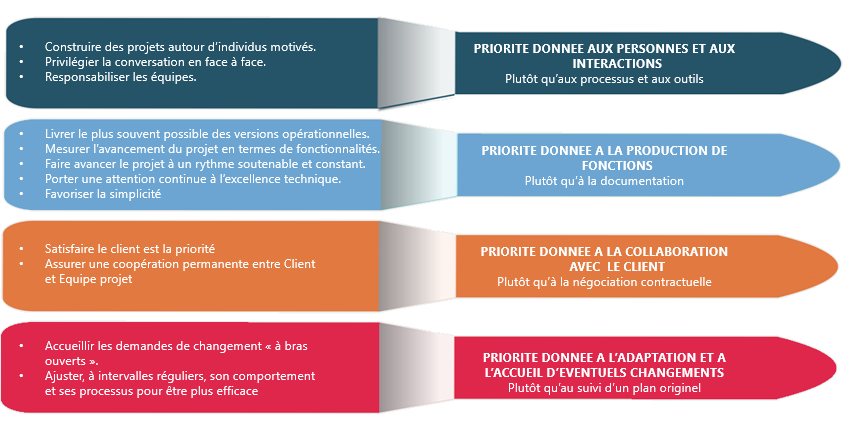
\includegraphics[width=1\columnwidth]{images/principes_agile.png}
\caption{les principes Agile}
\label{fig:les principes Agile}
\end{figure} 

\item \textbf{Processus de développement :}
Agile suit un développement de versions succes- \\ sives appelées incréments qui ajoutent et changent des fonctionnalités nécessaires au fil du temps pour fournir un produit plus robuste. Chaque module successif est planifié, codé, testé et complété sur de courtes sessions de deux à quatre semaines comme le montre la figure ci-dessous.
\begin{figure}[H]
\centering
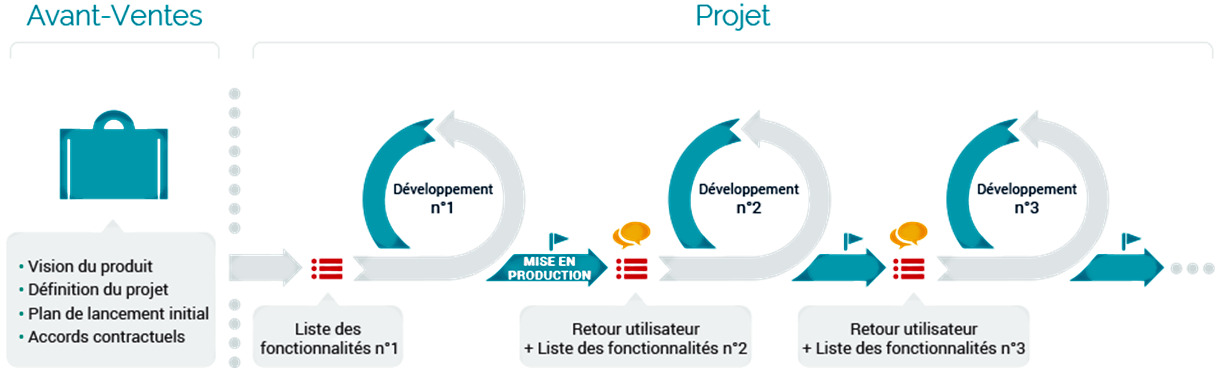
\includegraphics[width=1\columnwidth]{images/processus_agile.png}
\caption{cycle de vie Agile}
\label{fig:Mod-Enseig}
\end{figure} 
\end{itemize}

\subsection{SCRUM}
La méthode Scrum est la méthode agile la plus utilisée, éprouvée et documentée. Elle est considérée comme un cadre simple pour la gestion des projets complexes qui se base sur la transparence, l’adaptation et l’inspection. Elle s’appuie sur le découpage du projet en itérations, nommés sprints. Ce dernier représente des « user stories » à réalisées dans une durée fixe de 1 à 4 semaines.
Dans notre équipe scrum nous avons cinq rôles : 
\begin{itemize}[label=\textbullet,font=\normalsize]
\addtolength{\itemindent}{1cm}
\item \textbf{Le product owner : } le représentant officiel du client, il définit les besoins du produit et rédige les spécifications
\item \textbf{Le scrum master :} Chargé de veiller à la mise en application de la méthode et au respect de ses objectifs.
\item \textbf{ L’équipe de développement :} Les membres chargés de la réalisation du sprint et d’un produit utilisable en fin de sprint. 
\item \textbf{Le consultant fonctionnel :} Il veille sur la satisfaction des besoins client tout en couvrir tous les scénarios possibles.

\end{itemize}

\begin{figure}[H]
\centering
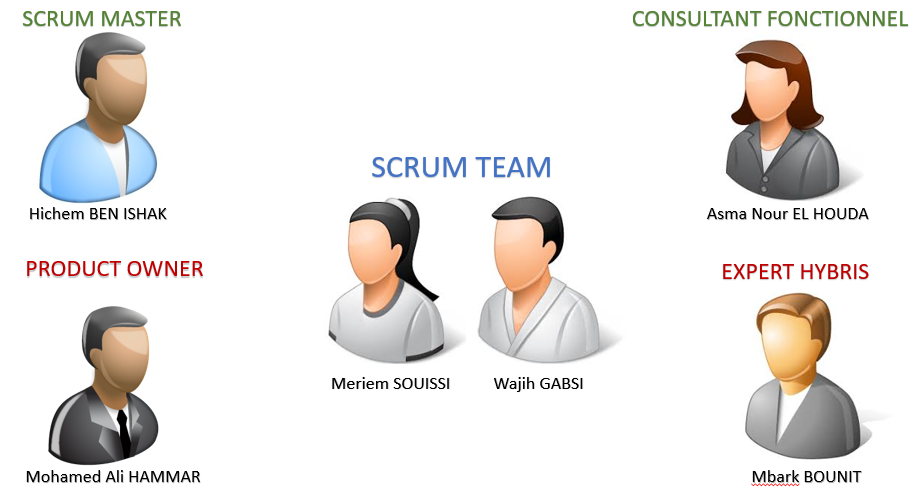
\includegraphics[width=0.7\columnwidth]{images/equipe_scrum.png}
\caption{équipe scrum}
\label{fig:Mod-Enseig}
\end{figure} 

En vue de bien mener les itérations, nous avons programmer pour chaque itération les réunions suivants :
\begin{itemize}[label=\textbullet,font=\normalsize]
\addtolength{\itemindent}{1cm}
\item \textbf{La planification du sprint }\\
Un « Sprint planning » est réalisé au début de chaque sprint, Mardi à quatorze heures. Durant cette réunion, nous décortiquons les cas d'utilisations présentés par le « product owner » en tâches techniques. Pour l’estimation des tâches, nous avons utilisé l’application mobile Scrum Poker 

\begin{figure}[H]
\centering
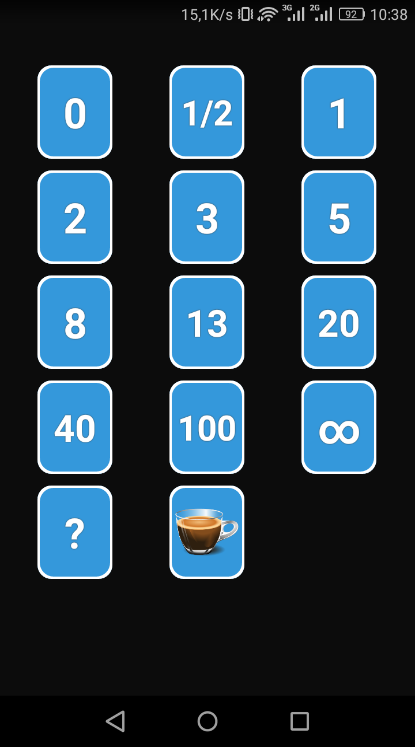
\includegraphics[width=0.29\columnwidth]{images/poker.png}
\caption{Scrum poker}
\label{fig:Mod-Enseig}
\end{figure} 

\item \textbf{La mêlée quotidienne}\\
Chaque matin nous assistons à la mêlée quotidienne pendant quinze minutes à neuf heures et quart. Durant cette réunion, le scrum master affiche le backlog produit et toute l’équipe répond chacun à ces trois questions :

\begin{itemize}[font=\normalsize]
\addtolength{\itemindent}{1cm}
\item Qu’est-ce que j’ai fait hier ? 
\item Qu’est-ce que je ferai aujourd’hui ?
\item Quels obstacles me retardent ?

\end{itemize}
\begin{figure}[H]
\centering
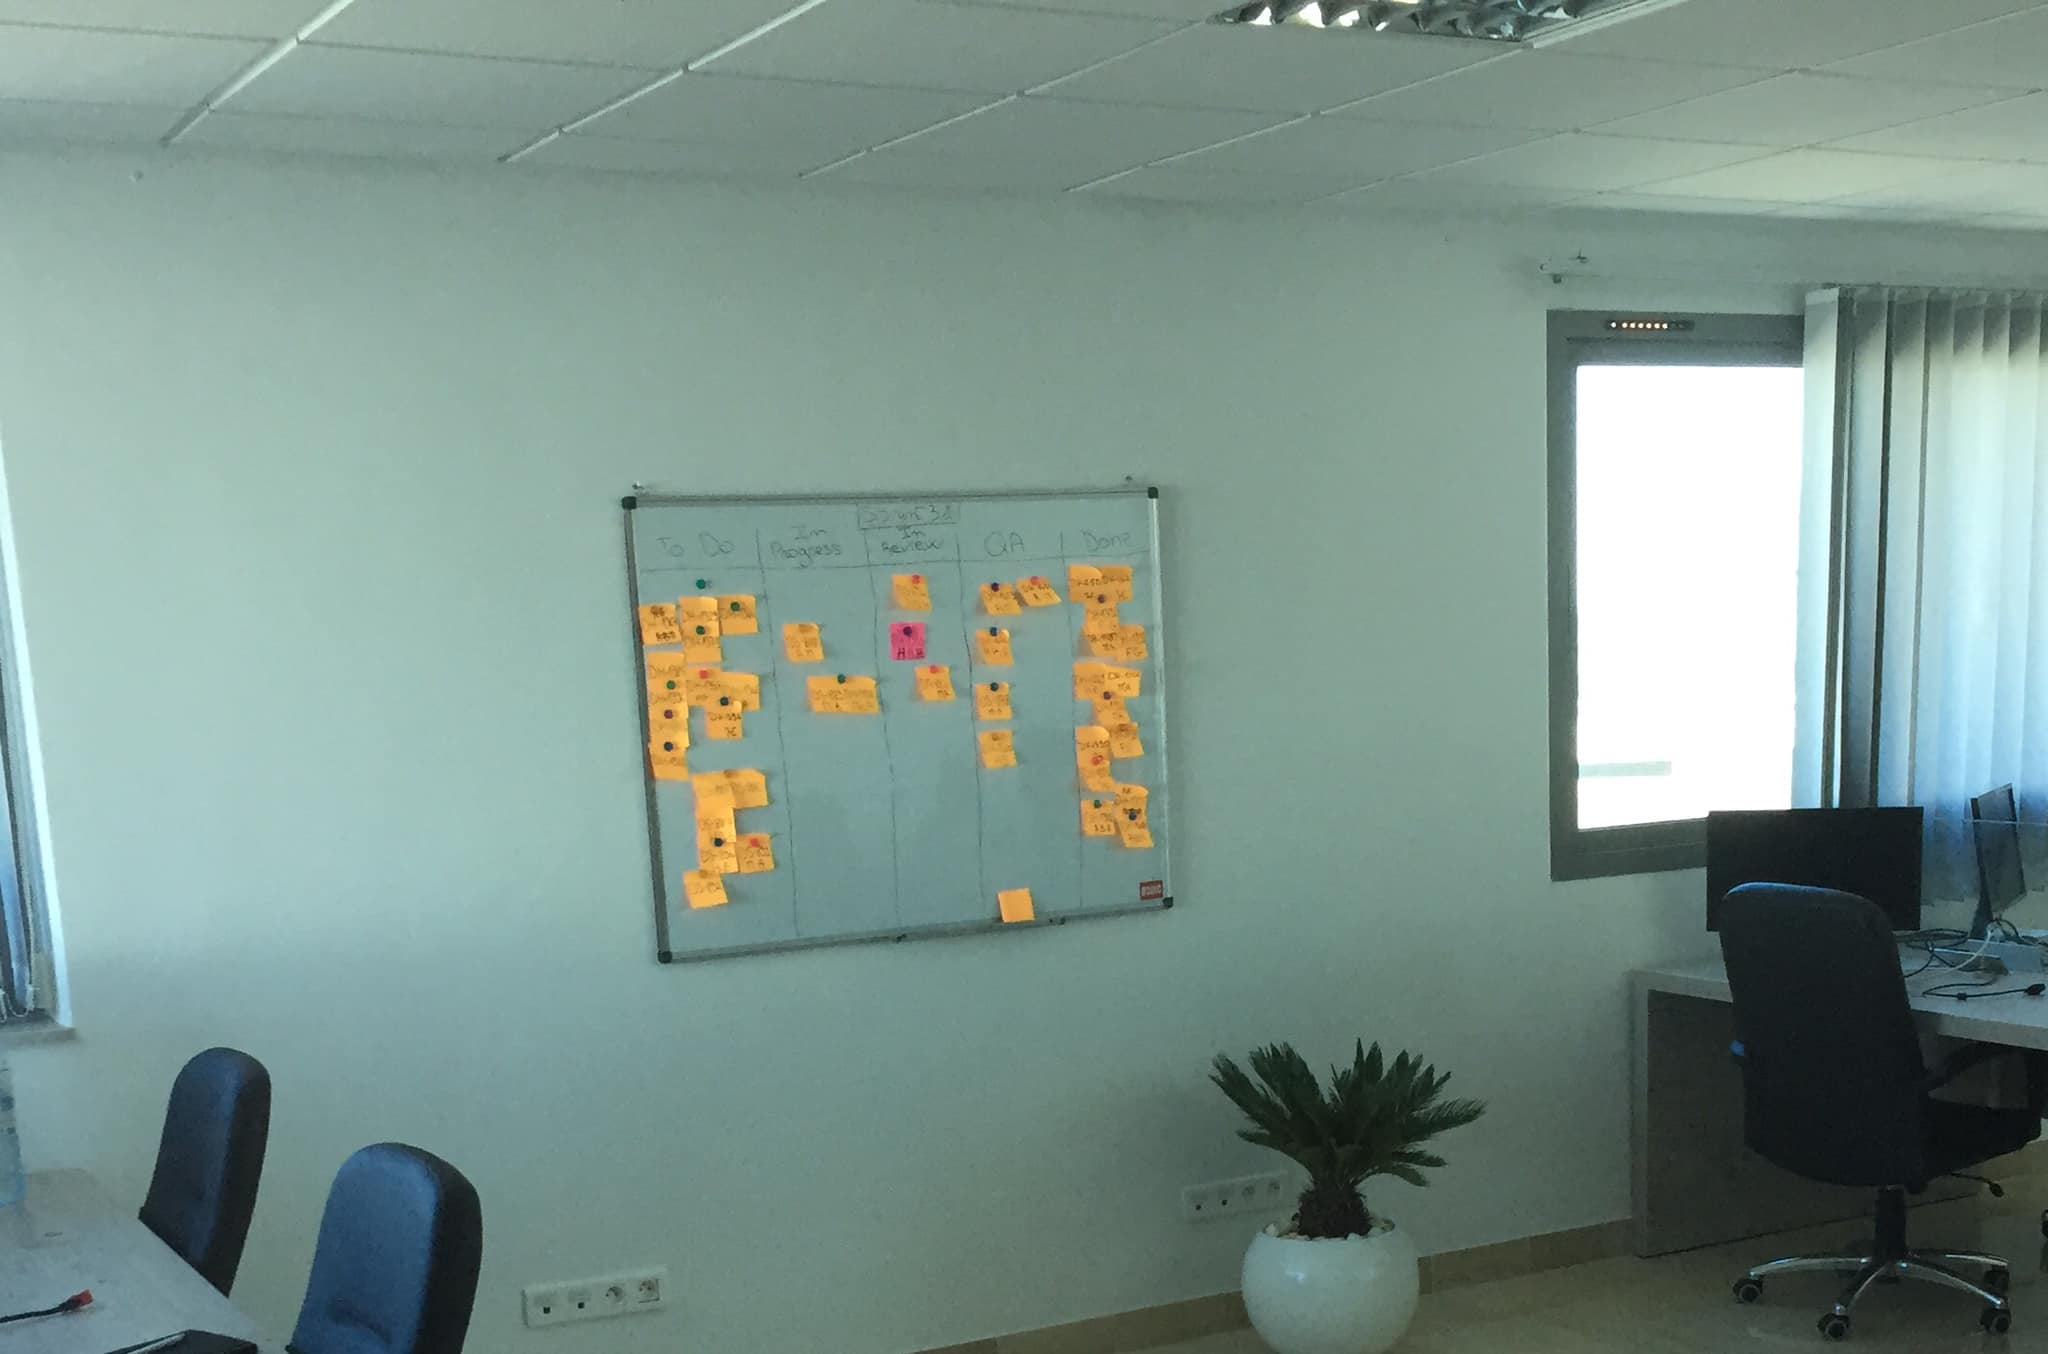
\includegraphics[width=1\columnwidth]{images/tableau1.jpg}
\caption{tableau des tâches}
\label{fig:tableau des Tâches}  
\end{figure}

\item \textbf{La revue du sprint}\\
À la fin de chaque sprint, tous les collaborateurs se réunissent pour la revue de sprint, chaque deux semaines, Le Mardi à dix heures. Durant cette réunion, nous discutons l’avancement du projet, nous évaluons les éléments finis et non finis et nous mettons à jour le Backlog produit.

\item \textbf{La rétrospective du sprint}\\
La réunion rétrospective se déroule une demi-heure juste après la revue de sprint en vue de faire le bilan de la période écoulée. Chacun évoque les points positifs et les points négatifs rencontrés tout au long du sprint.

Le schéma ci-dessous résume le processus scrum appliqué par notre équipe.

\begin{figure}[H]
\centering
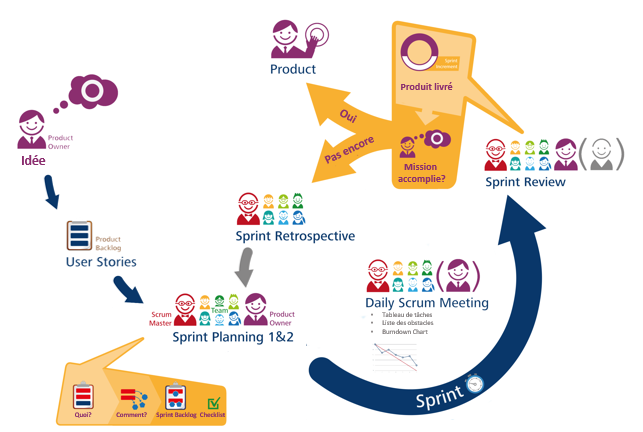
\includegraphics[width=1\columnwidth]{images/cycle_scrum.PNG}
\caption{processus scrum}
\label{fig:processus Scrum}
\end{figure} 
\end{itemize}

Notre équipe utilise l'outil Jira Agile pour la gestion du projet et des tickets, cela nous a permis de planifier et de suivre notre travail.
Les tâches sont exécutées comme suit :
Chaque tâche assignée par un membre de l’équipe doit être implémentée dans les délais définis. Ensuite nous planifions une revue de code avec un expert Hybris pour valider les spécifiés de Hybris. Si tout est validé, le code sera intégré. Finalement, la tâche sera assignée à la consultante fonctionnelle pour effectuer les tests fonctionnels nécessaires

Une tâche affectée à un développeur est une tâche en progression. Si elle est résolue, il fait un commit sur la branche d’intégration du GitLab. Dès lors, elle sera affecté au consultant fonctionnel qui doit faire les tests nécessaires, si ok elle sera validée, sinon elle sera « reopened ». Une tâche peut être en attente d'un autre évènement ou bloquée si nous n'avons pas trouvé une solution, Comme elle peut être rejetée.



\section{Les logiciels de suivi}

Pour gérer le cycle de vie du projet, nous disposons d’une chaine d’intégration continue basé sur le logiciel de suivi du projet Jira, le gestionnaire de versionning GitLab, et SonarLint l’outil de mesure de la qualité de code.

\textbf{Jira :} Le logiciel de suivi des projets, utilisé pour créer les « user stories » et les tâches. Il nous a permis aussi de planifier les sprints, d'affecter les tâches aux développeurs et d'exploiter l'avancement du développement en temps réel.

\textbf{GitLab :} Un outil dédié pour le gestionnaire de « versionning» , il permet la partage d'une base commune de travail entre les membres de l’équipe, le développement parallèle de plusieurs fonctionnalités et la gestion des conflits entre les développeurs. il permet en outre d'avoir des versions du code source sur des branches autre que la branche de déploiement.

\textbf{SonarLint :} SonarLint est un nouveau plugin officiel de SonarSource (première version datant d'octobre 2015) permettant l’analyse syntaxique du code source directement dans l'IDE en utilisant les règles d'analyse de SonarQube.
\newpage




\begin{figure}[H]
\centering
\frame{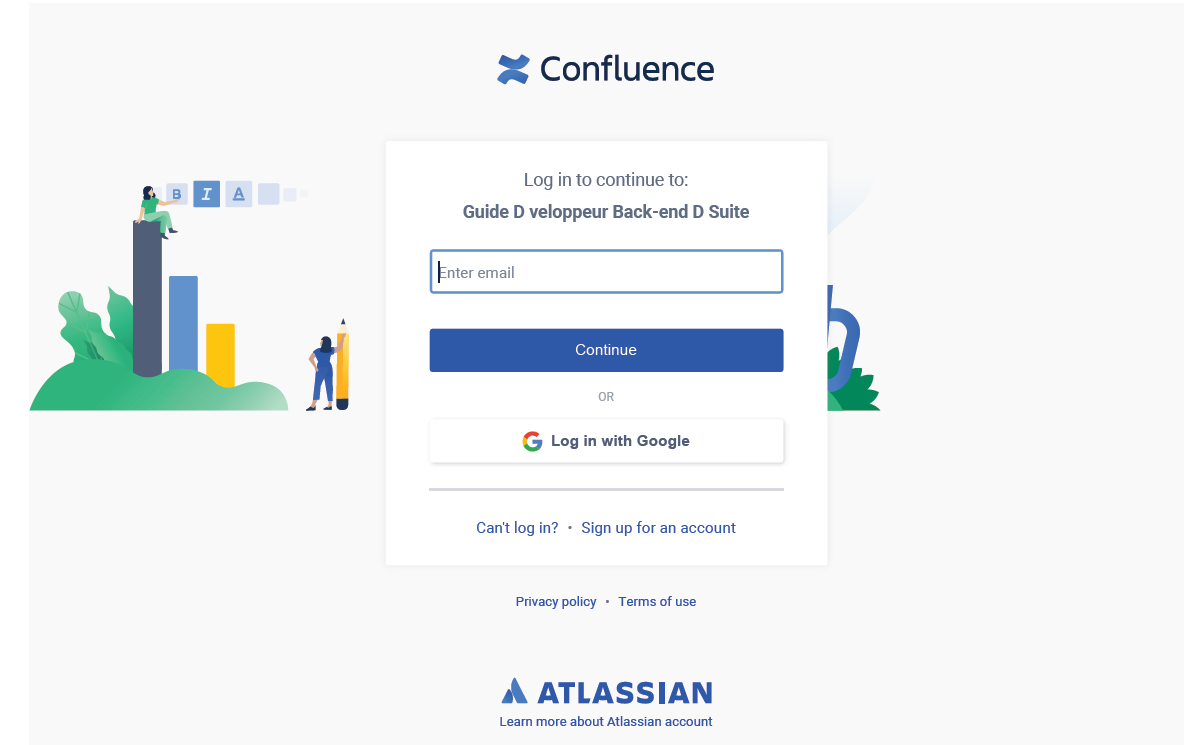
\includegraphics[width=1\columnwidth,height=0.6
\columnwidth]{images/Scrum.png}}
\caption{Jira}
\label{fig:Mod-Enseig}
\end{figure}

\section*{Conclusion}

\vspace{1cm \large Ce chapitre nous a donné l’occasion d’introduire les notions de bases de notre projet, nous avons présenté dans un premier lieu la société accueillante, puis nous avons mis le projet dans son contexte général. Puis nous avons fait une étude de l’état de l’art et enfin, nous avons établit les choix de la méthodologie appliquée dans notre projet.}

        \clearpage
        
        \chapter{État de l'art}

\section*{Inroduction}
    L'assurance, aujourd'hui, est devenue un bien de consommation courante, voire de première nécessité. Il suffit de recenser les assurances dont dispose en général le simple particulier dans sa vie quotidienne : assurance auto, multirisque habitation, santé, pour les plus fréquentes, auxquelles viennent s'ajouter les assurances vie, individuelle accidents, protection juridique, loisirs... Tout le monde en conviendra, l'assurance fait partie de la vie, En d'autres termes, pas de réalisation de projet sans assurance. 
    
\section{Assurance}
    \subsection{Définition de l'assurance}
    
                
        \begin{itemize}[font=\normalsize]
                \ding{226}\textbf{ Point de vue de l’Assuré : } L’assurance est une opération par laquelle un individu (l’Assuré) se fait promettre, contre rémunération de l’assureur (la Cotisation ou prime) à son profit ou à celui d’un tiers (le Bénéficiaire) en cas de réalisation de l’aléa prévu au contrat (le Risque)
                le versement d’une prestation (l’Indemnisation)
                par l’entreprise qui propose le contrat  \\
                
                \ding{226} \textbf{ Point de vue de l’Assureur :} 
                L’assurance
correspond au fait d’utiliser l’ensemble
des
Cotisations des Assurés ,
récoltées par
l’Assureur ,
afin de pouvoir verser
l’Indemnisation
au
Bénéficiaire en cas de
réalisation du
Risque .\\
                
                
        \end{itemize}
    
    \subsection{Les types des Assurances}
 \begin{figure}[H]
\centering
\frame{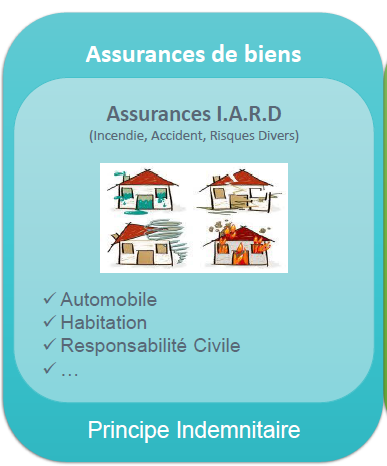
\includegraphics[width=0.5\columnwidth,height=0.4
\columnwidth]{images/Assurances_de_biens.png}}
\caption{Assurances de biens}
\label{fig:Mod-Enseig}
\end{figure}   

\begin{figure}[H]
\centering
\frame{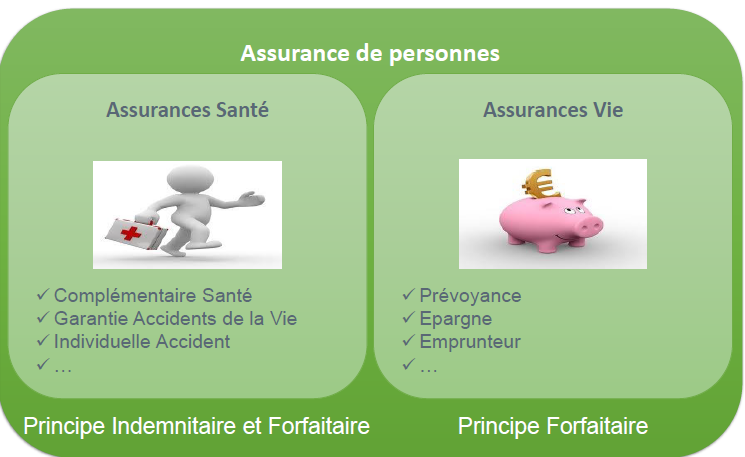
\includegraphics[width=0.5\columnwidth,height=0.4
\columnwidth]{images/Assurance_de_personnes.png}}
\caption{Assurance de personnes}
\label{fig:Mod-Enseig}
\end{figure}
\newpage
    
    \textbf{Principe Indemnitaire :}
    
    L’indemnité
due par l’assureur ne peut dépasser le
montant de la chose assurée au moment du sinistre
L’indemnité ne peut devenir une source d’enrichissement
de l’assuré
    
   
    \textbf{Principe Forfaitaire :}
    
    Le
montant du capital ou de la rente dû par l’assureur
est fixé par le contrat car le dommage subi ne peut
être évaluer objectivement.

\section{Les acteurs de l’assurance}    
    \subsection{Les Apporteurs (Réseaux de distribution)}
    \begin{figure}[H]
\centering
\frame{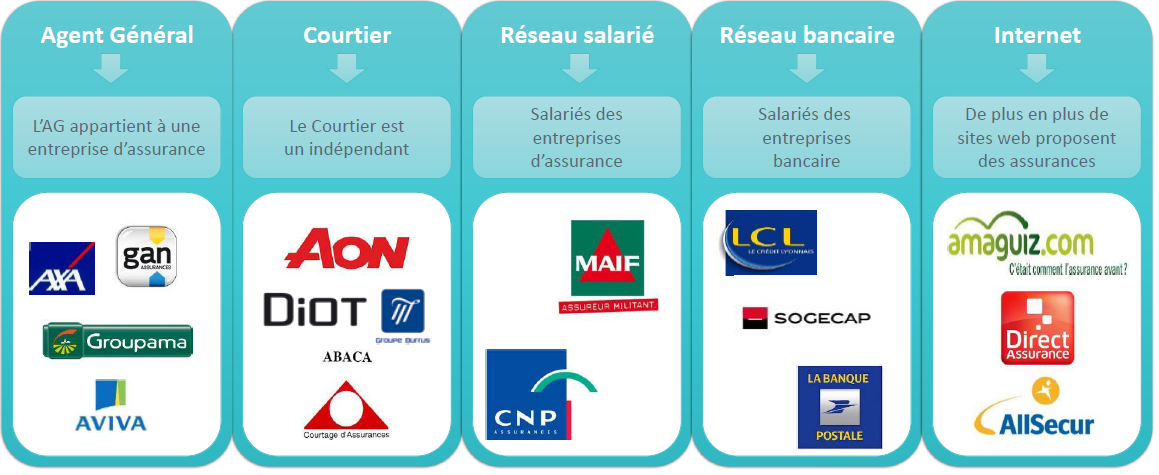
\includegraphics[width=1\columnwidth,height=0.6
\columnwidth]{images/les_acteurs_de_assurance.png}}
\caption{Les Apporteurs}
\label{fig:Mod-Enseig}
\end{figure}
       

    \subsection{Les Porteurs de Risques}
          \begin{figure}[H]
\centering
\frame{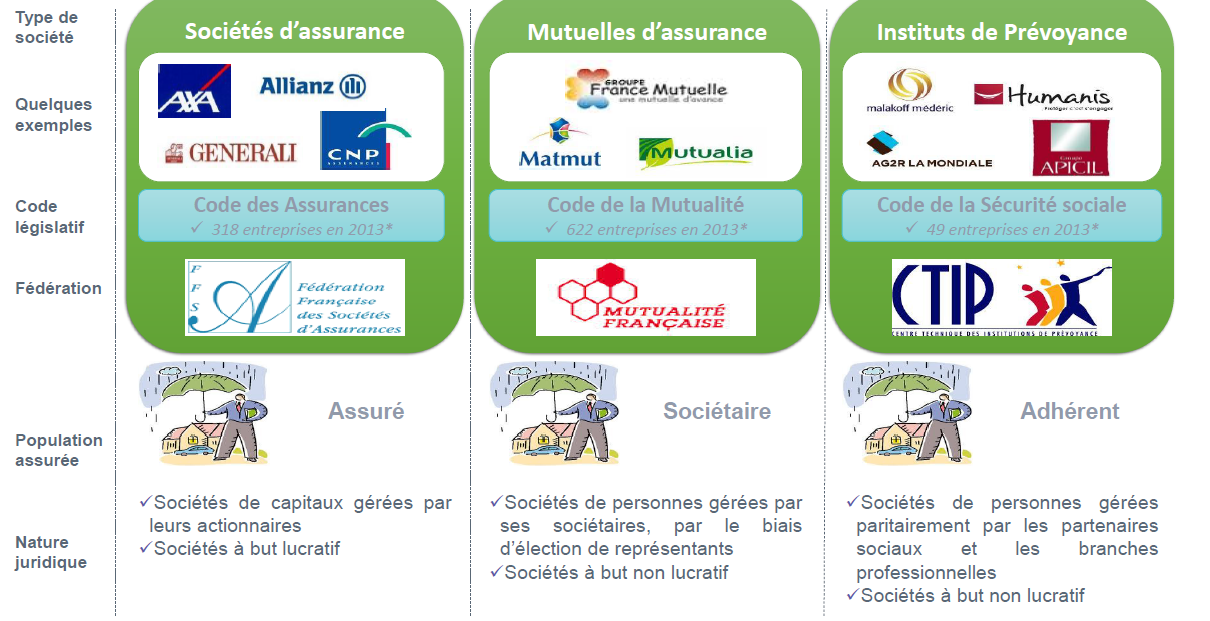
\includegraphics[width=1\columnwidth,height=0.6
\columnwidth]{images/les_porteurs_de_risques.png}}
\caption{Les porteurs de risque}
\label{fig:Mod-Enseig}
\end{figure}

          \begin{figure}[H]
\centering
\frame{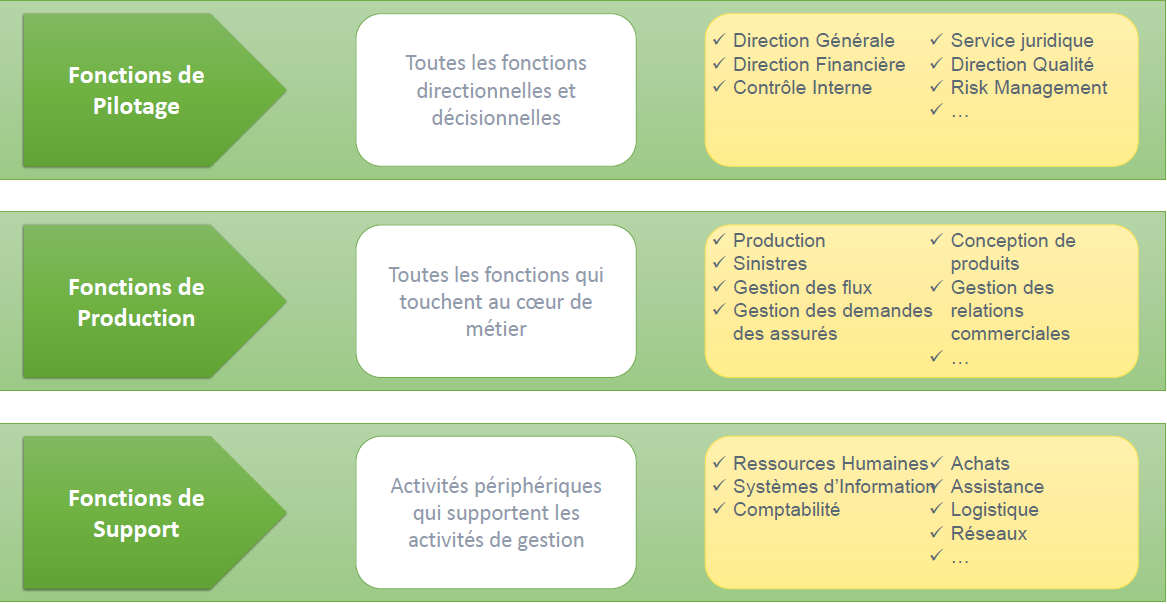
\includegraphics[width=1\columnwidth,height=0.6
\columnwidth]{images/les_porteurs_de_risques2.png}}
\caption{Les porteurs de risque}
\label{fig:Mod-Enseig}
\end{figure}
        

\newpage
    \section{Comprendre la Sécurité sociale}
    \subsection{Les 5 branches de la Sécurité sociale}
              \begin{figure}[H]
\centering
\frame{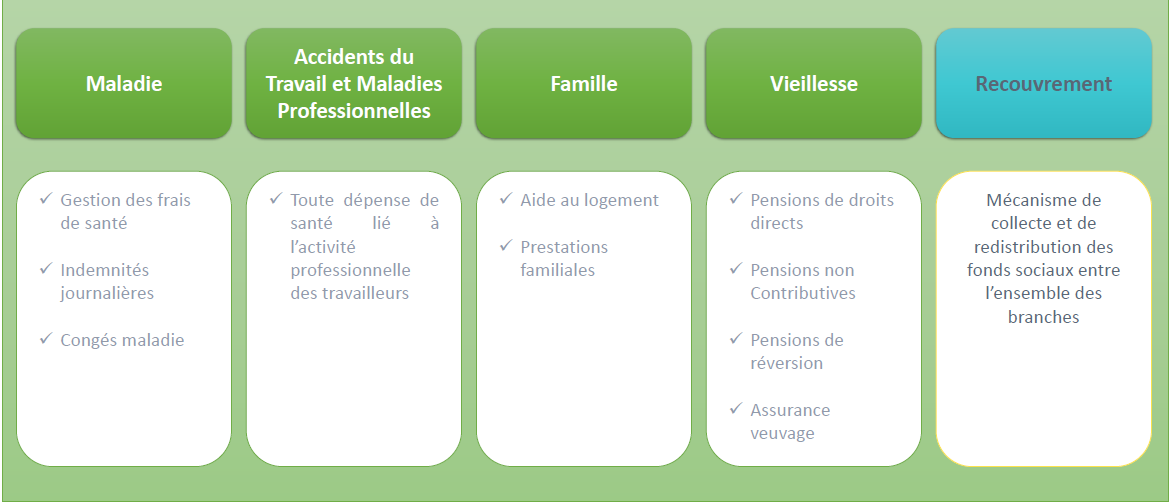
\includegraphics[width=1\columnwidth,height=0.6
\columnwidth]{images/les5.png}}
\end{figure}
    
        
        
    \subsection{Les grands régimes de la Branche Maladie}
    
    L’Assurance Maladie Obligatoire est constituée de trois principaux régimes:
    \begin{itemize}[font=\normalsize]
                \ding{226}\textbf{ Le
régime général (regroupe environ 4 personnes sur 5) }\\
\end{itemize}
\begin{itemize}[font=\normalsize]
                \ding{226}\textbf{ Le
régime des salariés agricoles }\\
\end{itemize}
\begin{itemize}[font=\normalsize]
                \ding{226}\textbf{ Le
régime social des indépendants }\\
\end{itemize}
    
    
    
               \begin{figure}[H]
                \centering
                \frame{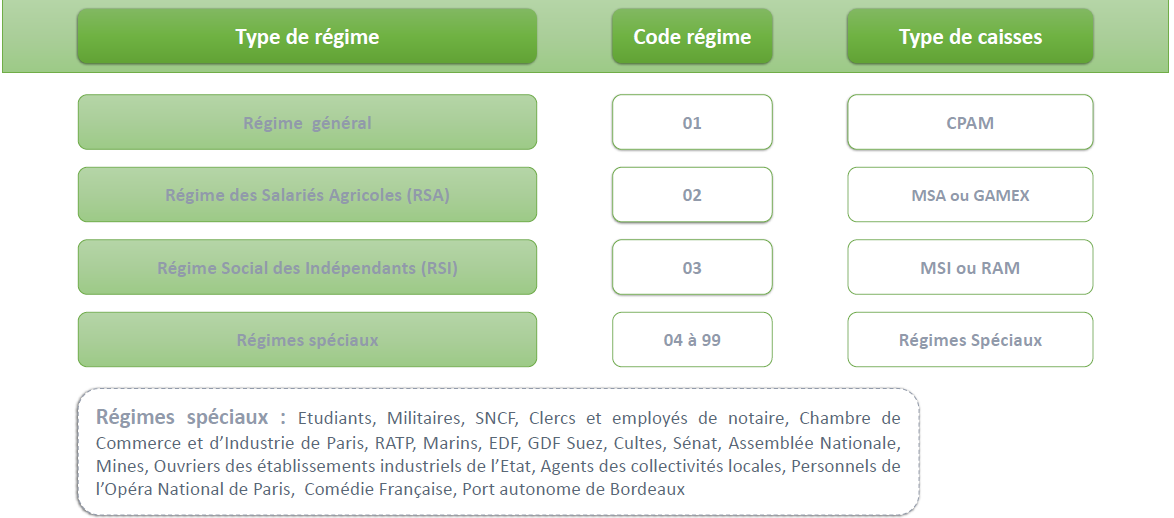
\includegraphics[width=1\columnwidth,height=0.6
                \columnwidth]{images/les6.png}}
                \end{figure}
    
        
    \subsection{Les principes de l’assurance santé}
    \begin{figure}[H]
                \centering
                \frame{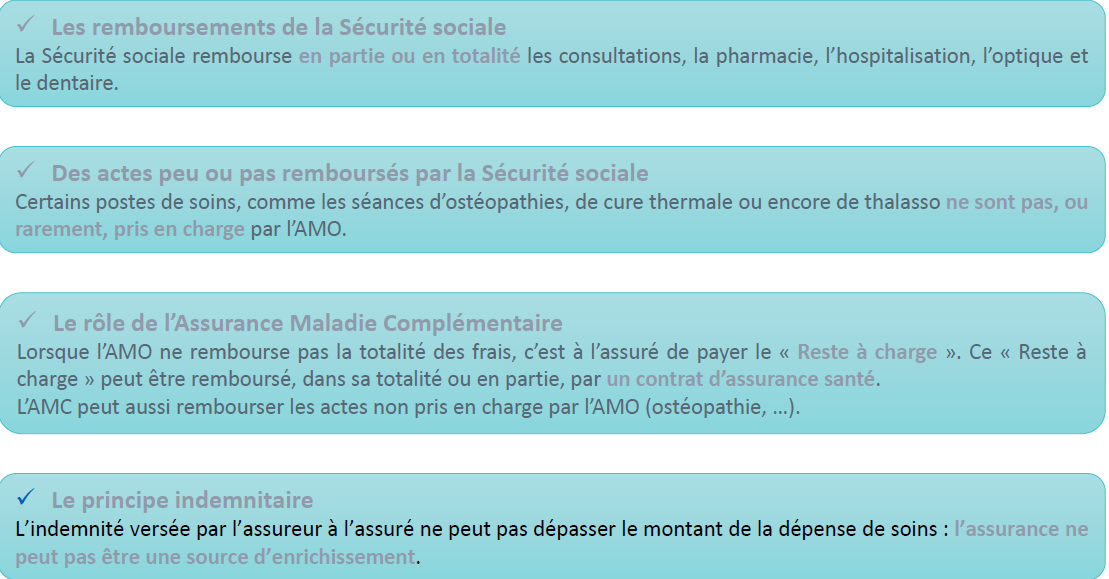
\includegraphics[width=1\columnwidth,height=0.6
                \columnwidth]{images/les7.png}}
                \end{figure}

   \section{Synthèse}
   \begin{figure}[H]
                \centering
                \frame{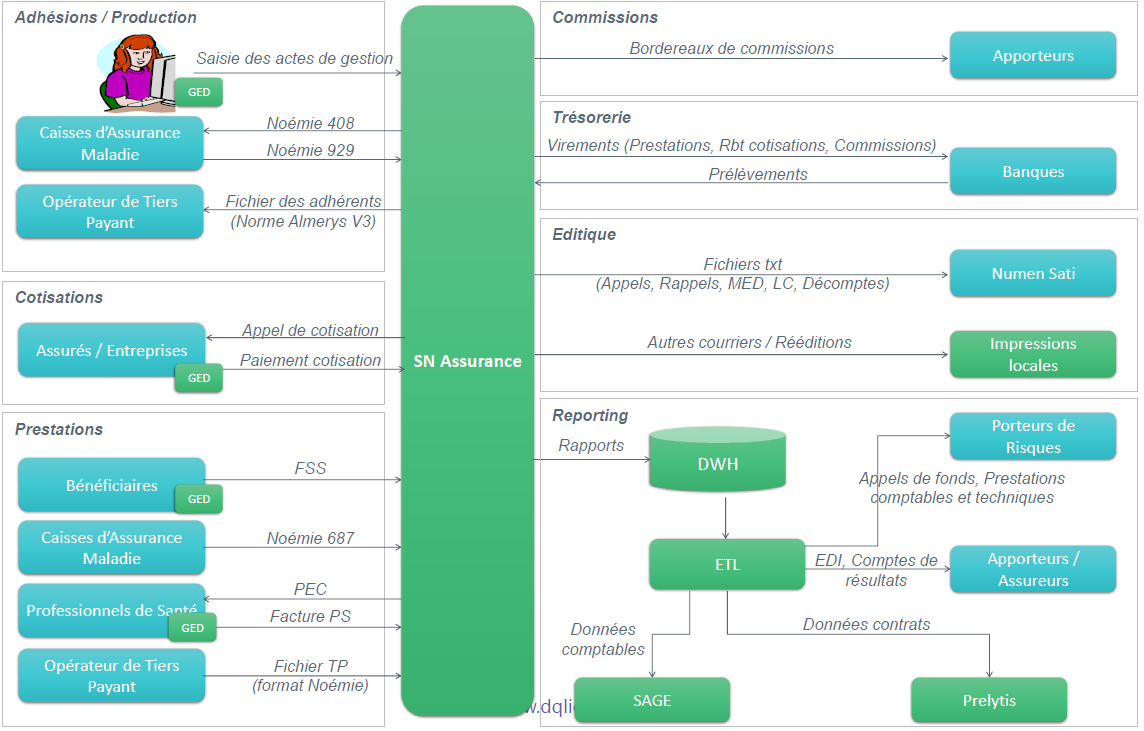
\includegraphics[width=1\columnwidth,height=0.7
                \columnwidth]{images/les8.png}}
                \end{figure}
          
    


\section*{Conclusion}
Dans ce chapitre, nous avons effectué une étude sur les différents aspects de l'assuarnce et sur les solutions existentes sur le marché national et global. Dans le chapitre suivant, nous allons dégager les besoins de nos utilisateurs en se basant sur cet étude. 
        \clearpage
        
        \chapter{Sprint0: Analyse et spécification des besoins}

%%% %%%%%%%%% %%%
\section*{Introduction}
Après аvoir présenté le cadre général et la méthodologie agile utilisée durant notre projet, nous présentons le sprint 0 qui a duré 2 semaines. Dans cette partie de ce chapitre, nous présentons les besoins fonctionnels et non fonctionnels du projet.
%%%%%%%%%%
\section{Analyse et spécification des besoins}
Dans cette partie, nous commençons par présenter tous les besoins que notre projet tourne autour desquels et qu’il doit les satisfaire. Ensuite, nous allons introduire les exigences fonctionnelles et non-fonctionnelles, et le diagramme de cas d’utilisation générаle.
\subsection{Besoins fonctionnels}
Le système réalisé dans le cadre de ce projet doit offrir à l’administrateur les possibilités suivantes :
\newpage
                \begin{itemize}
                \item Accélérer la distribution de l’offre en fluidifiant les parcours, de la mise en marché à la vente multicanal.
                \item Simplifier les processus de gestion et l’expérience de l’assuré.
                \item Enrichir cette expérience en proposant de nouveaux services digitaux répondant aux nouveaux usages.
                \end{itemize}



\subsection{Diagrammes de cas d’utilisation général}
Après avoir dégagé les différents acteurs en interaction avec notre système et les exigences fonctionnels et non fonctionnels, nous allons présenter ces différentes fonctionnalités avec le diagramme de cas d’utilisation général 
\begin{figure}[H]
\centering
\frame{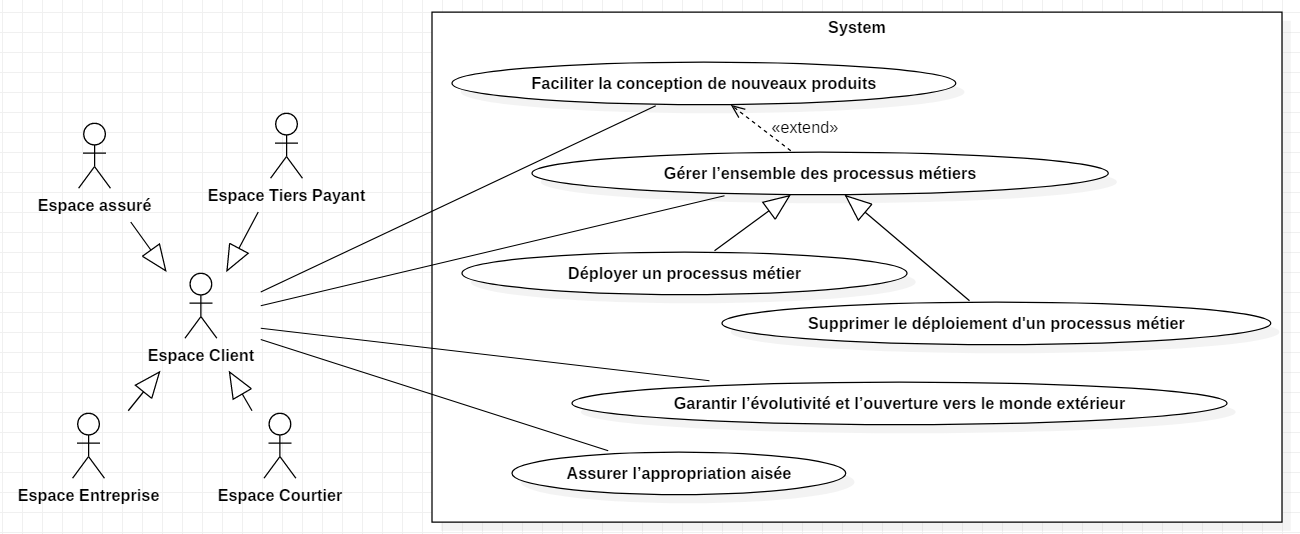
\includegraphics[width=1.1\columnwidth,height=0.7
\columnwidth]{images/use.png}}
\caption{Diagramme de cas d’utilisation général}
\end{figure}

\subsection{Besoins non-fonctionnels}
Les besoins non fonctionnels décrivent toutes les contraintes techniques, ergonomiques et esthétiques auxquelles est soumis le système pour sa réalisation et pour son bon fonctionnement. Et ce qui concerne notre application, nous avons dégagé le besoins suivants :

\begin{itemize}[font=\normalsize]
                \ding{226}\textbf{Fiabilité et pertinence :} les services doivent fournir des résultats corrects et pertinents.
                \end{itemize}
\begin{itemize}[font=\normalsize]
                \ding{226}\textbf{Temps réel :} la solution doit fournir les ressources demandées en temps réel.
                \end{itemize}
\begin{itemize}[font=\normalsize]
                \ding{226}\textbf{Maintenаbilité :} la maintenabilité et l’évolutivité sont obligаtoires pour avoir un logiciel de qualité.
                \end{itemize}
\begin{itemize}[font=\normalsize]
                \ding{226}\textbf{Lisibilité d’un code source :} Le code de l’applicаtion doit être lisible et compréhensible afin de garantir la maintenance de l’application en cas de besoin.
                \end{itemize}
\begin{itemize}[font=\normalsize]
                \ding{226}\textbf{Performance :} le système doit être stable et son temps de réponse doit être tolérable.
                \end{itemize}
\begin{itemize}[font=\normalsize]
                \ding{226}\textbf{Ergonomie :} L’interface utilisateur doit être claire et facile à manipuler
                \end{itemize}

\section{L’architecture logique}
\subsection{D Health}
\subsubsection{\Large Pour Qui ?}
D HEALTH est dédié aux assureurs traditionnels, aux mutuelles, aux
courtiers, distributeurs, banques, sociétés de gestion et institutions
de prévoyance.
D HEALTH couvre toute la chaîne de valeur (Clients, Partenaires,
Distributeurs, Gestionnaires, Tiers) , en plus des fonctionnalités
basiques D HEALTH permet également de :
\begin{itemize}[font=\normalsize]
                \ding{226}\textbf{Faciliter la conception de nouveaux produits }
                
\end{itemize}
\begin{itemize}[font=\normalsize]
                \ding{226}\textbf{Permettre la configuration de l’ensemble des processus métiers}
                \end{itemize}
                \begin{itemize}[font=\normalsize]
                \ding{226}\textbf{Garantir l’évolutivité et l’ouverture vers le monde extérieur}
                \end{itemize}
                \begin{itemize}[font=\normalsize]
                \ding{226}\textbf{Assurer l’appropriation aisée par les utilisateurs du système
d’information}
                \end{itemize}
                \subsubsection{Nos Atouts ?}
                \begin{itemize}[font=\normalsize]
                 \ding{226}\textbf{la performance :} robustesse, traçabilité ...
                 \end{itemize}
                 \begin{itemize}[font=\normalsize]
                  \ding{226}\textbf{la sécurité et conformité réglementaire}
                  \end{itemize}
                  \begin{itemize}[font=\normalsize]
                   \ding{226}\textbf{la flexibilité du modèle :} SaaS, PaaS ou IaaS
                   \end{itemize}
                   \begin{itemize}[font=\normalsize]
                    \ding{226}\textbf{l’innovation :} Ateliers produits,
User expérience,
OCR,
workflows paramétrables,
détection de la fraude,
Contrôle de la qualité des données.
                    \end{itemize}
                    \begin{itemize}[font=\normalsize]
                     \ding{226}\textbf{User Expérience}
                     \end{itemize}
                     
                \begin{figure}[H]
\centering
\frame{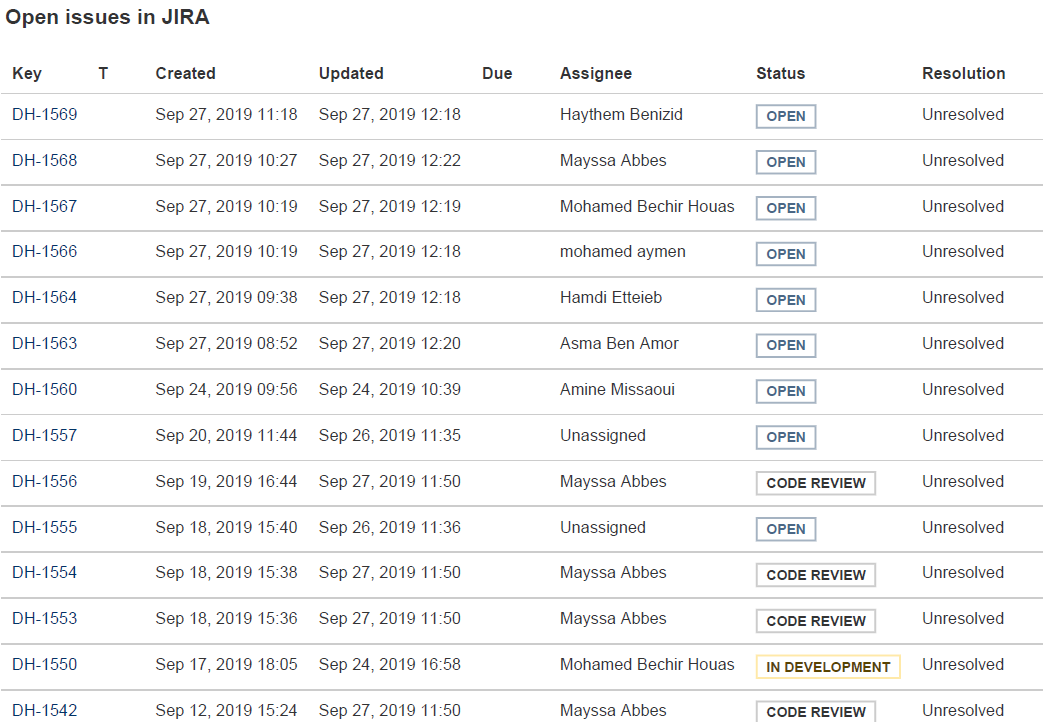
\includegraphics[width=1\columnwidth,height=0.6
\columnwidth]{images/les9.png}}
\caption{Open issues in JIRA}
\label{fig:Mod-Enseig}
\end{figure}
                      
\subsection{D Suite}     
Dans un contexte économique de plus en plus concurrentiel, les acteurs de l’assurance sont confrontés à une clientèle exigeante,
renseignée et plus volatile. Depuis la mise en vigueur de la loi Hamon et le développement des comparateurs d’assurance, les assurés ont la
possibilité de changer de prestataire d’assurance en un claquement de doigts.
Pour anticiper et se prémunir de la fuite de leurs clients, les assureurs mettent en place des solutions de gestion de la relation client permettant
de répondre à une politique de satisfaction plus stricte. Afin de rendre cet objectif atteignable, les acteurs de l’assurance développent une
stratégie d’accompagnement des assurés depuis la souscription d’un contrat jusqu’à sa résiliation.
D Suite d'outils et d'application web proposée par Dqlick qui est  compatible avec D Health et qui touchent plusieurs domaines :

\begin{itemize}[font=\normalsize]
                 \ding{226}\textbf{Espace assuré}
                 \end{itemize}
                 \begin{itemize}[font=\normalsize]
                  \ding{226}\textbf{Espace Entreprise}
                  \end{itemize}
                  \begin{itemize}[font=\normalsize]
                   \ding{226}\textbf{Espace Courtier}
                   \end{itemize}
                   \begin{itemize}[font=\normalsize]
                    \ding{226}\textbf{Espace Tiers Payant}
                 \end{itemize}
                 \begin{itemize}[font=\normalsize]
                  \ding{226}\textbf{Outil aide à la vente}
                  \end{itemize}
                  \begin{itemize}[font=\normalsize]
                   \ding{226}\textbf{E-Devis}
                   \end{itemize}
                   \begin{itemize}[font=\normalsize]
                  \ding{226}\textbf{GED}
                  \end{itemize}
                  \begin{itemize}[font=\normalsize]
                   \ding{226}\textbf{Espace Administration des assurés}
                   \end{itemize}
                   
                                   \begin{figure}[H]
\centering
\frame{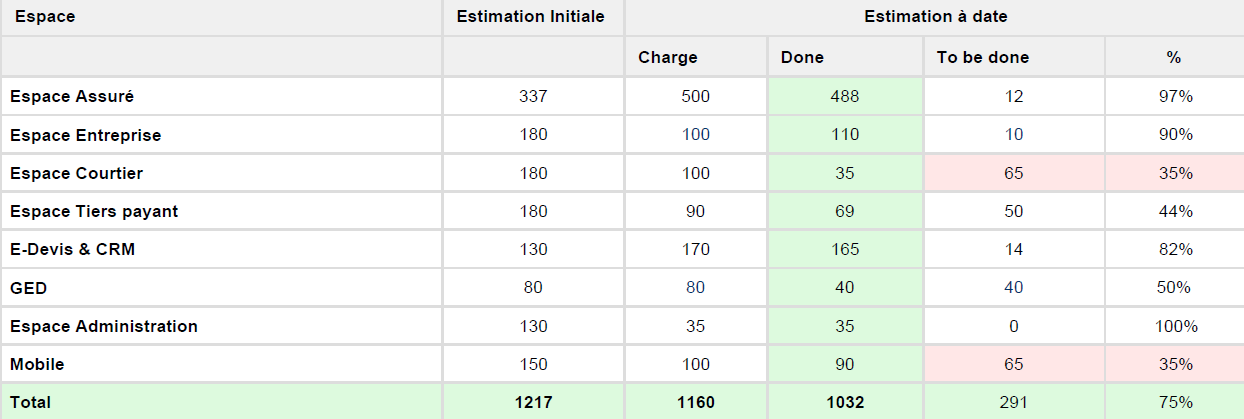
\includegraphics[width=1\columnwidth,height=0.6
\columnwidth]{images/les10.png}}
\caption{Gestion Projet}
\label{fig:Mod-Enseig}
\end{figure}
                                   \begin{figure}[H]
\centering
\frame{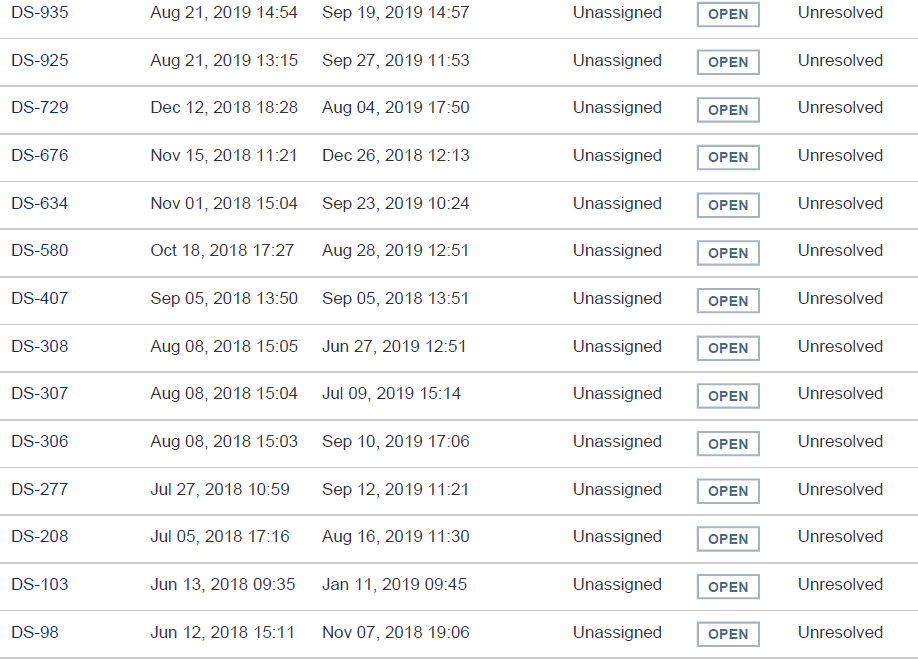
\includegraphics[width=1\columnwidth,height=0.6
\columnwidth]{images/les11.png}}
\caption{Open issues in JIRA}
\label{fig:Mod-Enseig}
\end{figure}
                   



\section*{Conclusion}
Dans ce chapitre nous avons identifié les besoins fonctionnels et non fonctionnels de notre projet. Nous avons construit l’architecture logique
D Health et D Suite de notre solution.
        \clearpage
        
        \chapter{Etude technique}

\section*{Inroduction}

\vspace{1cm \large Dans cette section, nous présentons en premier lieu l’architecture microservices et son utilité dans le monde informatique moderne. Puis, nous indiquons les technologies que nous utilisons pour réaliser notre travail ainsi que l’environnement de développement.}

\section{Architecture micro-services}

\vspace{1cm\large Micro-services est un style architectural qui représente un moyen de
concevoir les applications comme ensemble de services indépendamment
déployables. Ces services doivent de préférence être organisés autours des
compétences métier, de déploiement automatique, d'extrémités intelligentes et
de contrôle décentralisé des technologies et des données.}

\begin{figure}[H]
    \centering
    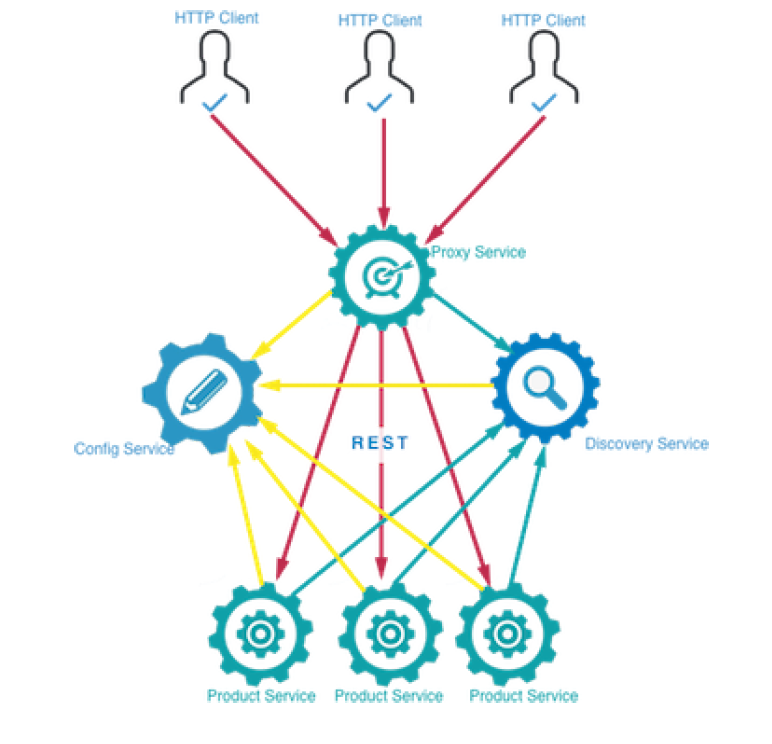
\includegraphics[width=0.7\columnwidth]{images/les12.PNG}
    \caption{Achitecture Microservice}
    \label{fig:Global}  
    \end{figure}
    \itemindent\textbf {\underline{Architecture}}
Cette architecture aborde le problème de la complexité
en décomposant l'application en un ensemble de services gérables qui sont beaucoup plus rapides
à développer et beaucoup plus faciles à comprendre et à maintenir. Cette architecture permet le développement de chaque service indépendamment l’un des autres par plusieurs équipes. De plus, elle réduit la barrière de l’adoption de nouvelles technologies puisque les développeurs sont libres de
choisir les technologies et ne sont pas limités aux choix faits au début du projet.
L’architecture microservices permet à chаque microservice d’être déployé indépendаmment. En conséquence, il rend possible le déploiement continu pour des applications complexes.

 \section{Technologies utilisées}
 \subsection{Les langages et Frameworks}
 Nous exposons, dans cette partie, les framework et les solutions technologiques nécessaires à la réalisation de notre projet et ce afin de satisfaire nos besoins fonctionnels et non fonctionnels.
 
 \begin{table}[H]
    \captionsetup{justification=centering}
    \caption{  \label{tab:UC-ATH} Tableau résumant les technologies utilisées dans notre projet.}
    \centering
    \begin{tabular} {|m{10em}|m{25em}|}
    \hline
    \rowcolor[HTML]{8c9eff} 
    \textbf{ } & \textbf{Technologie} \\
    \hline
    \rowcolor[HTML]{e8eaf6}
    \textbf{Backend} & JAVA8, SPRING BOOT, SPRING CLOUD, MAVEN, Bamboo \\
    \hline
    \rowcolor[HTML]{f3e5f5}
    \textbf{Frontend} & Angular, HTML5, CSS3 et Typescript. \\
    \hline
    \rowcolor[HTML]{e8eaf6}
    \textbf{BDD} & NoSQL, Cassandra \\ 
    \hline
    \rowcolor[HTML]{f3e5f5}
    \textbf{Méthodologies} & Agile SCRUM. \\ 
    \hline
    \rowcolor[HTML]{e8eaf6}
    \textbf{DEVOPS} & JIRA, GitLab, SonarLint.\\
    \hline
    \end{tabular}
    \end{table}
    
    \subsubsection{JAVA8}
    Java 8 est la dernière version stable de Java qui offre de nouvelles fonctionnalités, desperformances accrues et des corrections de bug pour améliorer l’efficacité de développementet d’exécution des programmes Java.Les nouvelles fonctionnalités de Java 8 :\\
    \noindent \textbf{-Expression lambda et méthodes d’extension virtuelle :} programmation fonctionnellepour un code plus simple et plus compact.\\
    \noindent \textbf{-API de date/heure :} facilite la gestion de la date et de l’heure de façon plus naturelle,simple et compréhensible.\\
     \noindent \textbf{-fMoteur JavaScript Nashorn :}exécution du code Javascript dans Java.\\
   \noindent \textbf{-Encodage Base64 :}pour la sécurité.\\
     \subsubsection{SPRING BOOT}
    
    Spring est le framework de développement d’applications le plus populaire. Il est né de l’idée de fournir une solution plus simple et plus légère que celle proposée par Java 2 EE. permet de son côté de construire des applications Spring rapidement aussi rapidement que possible, en minimisant au maximum le temps de configuration, d'habitude
pénible.

                  
                  \subsubsection{ANGULAR}
                  Angular est une plateforme de développement qui permet de créer des applications web dynamiques et immersives.  Dans ce cours, vous apprendrez rapidement à créer les composantes de base d'une application Angular, avant d'enrichir vos applications en approfondissant vos connaissances de ce framework.  Vous apprendrez également à faire communiquer votre application avec un backend afin de créer une application web complète.
                  
                   \subsubsection{Cassandra (base de données)}
                   Apache Cassandra est un système de gestion de base de données (SGBD) de type NoSQL conçu pour gérer des quantités massives de données sur un grand nombre de serveurs, assurant une haute disponibilité en éliminant les points individuels de défaillance. Il permet une répartition robuste sur plusieurs centres de données4, avec une réplication asynchrone sans master et une faible latence pour les opérations de tous les clients.
                   \subsubsection{Bamboo}
                   Bamboo est un outil Open-Source d’Intégration Continue, le principe est de vérifier, idéalement à chaque modification de code source, que le
résultat de ces modifications de produit pas de régression sur l’application, la mise en commun entre développeurs se fait à chaque
modification/commit, en continu ; ce qui permet d’augmenter les chances que chaque portion de l’application fonctionne avec ses autres
composantes.
                  
                  
































    \subsection{Environnement logiciel}
    
    \subsubsection{Spring Tool Suite (STS 4): Backend}
    
   STS est un environnement de développement basé sur Eclipse qui est personnalisé pour le développement d'applications Spring.

Il fournit un environnement prêt à l'emploi pour implémenter, déboguer, exécuter et déployer vos applications. Il inclut également une intégration pour Pivotal tc Server, Pivotal Cloud Foundry, Git, Maven et AspectJ. STS s’ajoute aux dernières versions d’Eclipse.
    
    \subsubsection{WebStorm 11: Frontend}
    WebStorm est un IDE pour les langages Web (HTML, CSS et JavaScript), développé par l'entreprise JetBrains et basé sur la plateforme IntelliJ IDEA
    

    
    \subsubsection{JIRA}
    
    C’est un logiciel pour la gestion de projets pour les équipes agiles. Il permet de gérer le backlog produit, les sprints ainsi que les tickets. De plus il permet d’établir des rapports pour se bénéficier des informations en temps réel par rapport à l’avancement et du temps consommé par tâche .
    
    \subsubsection{SourceTree}
    SourceTree simplifie la façon dont vous interagissez avec vos référentiels Git afin que vous puissiez vous concentrer sur le codage. Visualisez et gérez vos référentiels via une interface simple.
    
    \subsubsection{DevCentre}
    DataStax DevCenter est un IDE visuel gratuit de schémas et de requêtes destiné aux développeurs, administrateurs et autres personnes souhaitant créer et exécuter des instructions CQL (Cassandra Query Language) sur Apache Cassandra et DataStax Enterprise. Les utilisateurs peuvent rapidement ajouter et créer de nouvelles connexions, importer des requêtes précédemment enregistrées et naviguer dans des instances de base de données. 
    
     \subsubsection{Postman}
Postman est un logiciel qui se focalise sur les tests des API. Il est devenu très populaire pour tester les Microservices, notamment grâce à sa simplicité et ses fonctionnalités très spécialisées.
\subsubsection{StarUML}
C’est un logiciel de modélisation qui prend en charge la modélisation agile. Il offre la
possibilité de modéliser plusieurs types de diagrammes tel que le diagramme de cas d’utilisation,
diagrammes de séquences et diagrammes de classes


\section{Architecture de l'environnement du travail}
    \subsection{Architecture physique}
    Pour l'architecture physique de notre projet, nous avons décidé de mettre en place une architecture microservice, c'est l'architecture qui convient le mieux avec nos besoins. 
Nous allons donc créer les microservices suivants:
\begin{itemize}[font=\normalsize]
                  \ding{226}\textbf{ Product Service :}Service principal, qui offre une API REST pour lister une
liste de produits
                  \end{itemize} .
                  
                  \begin{itemize}[font=\normalsize]
                  \ding{226}\textbf{ Config Service :}Service de configuration, dont le rôle est de centraliser les
fichiers de configuration des différents microservices dans un endroit
unique.
                  \end{itemize} .
                  \begin{figure}[H]
        \centering
        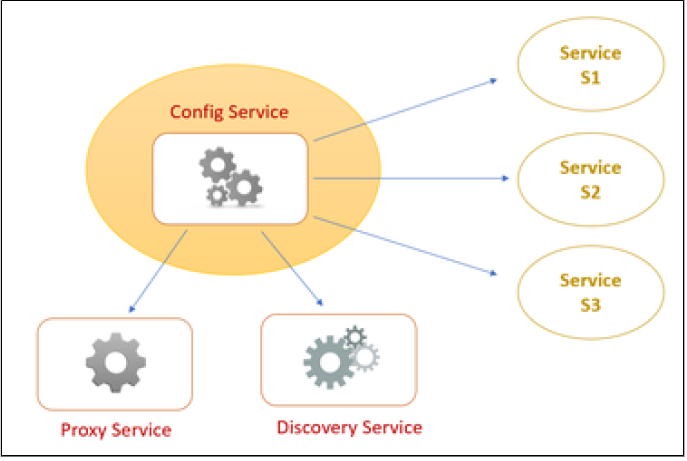
\includegraphics[width=1\columnwidth,height=0.5
\columnwidth]{images/config.PNG}
        \caption{Microservice Config-Service}
        \end{figure}
        \newpage
        
                  \begin{itemize}[font=\normalsize]
                  \ding{226}\textbf{ Proxy Service :}Passerelle se chargeant du routage d'une requête vers l'une
des instances d'un service, de manière à gérer automatiquement la
distribution de charge.
                  \end{itemize} 
                   \begin{figure}[H]
        \centering
        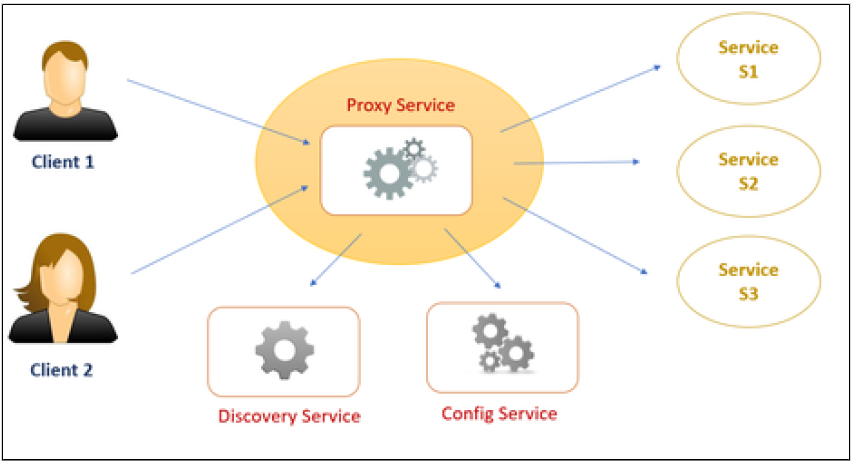
\includegraphics[width=1\columnwidth,height=0.4
\columnwidth]{images/proxy.PNG}
        \caption{Microservice Proxy-Service}
        \end{figure}.
                  \begin{itemize}[font=\normalsize]
                  \ding{226}\textbf{ Discovery Service :}Service permettant l'enregistrement des instances de
services en vue d'être découvertes par d'autres services.
                  \end{itemize} .
                  \begin{figure}[H]
        \centering
        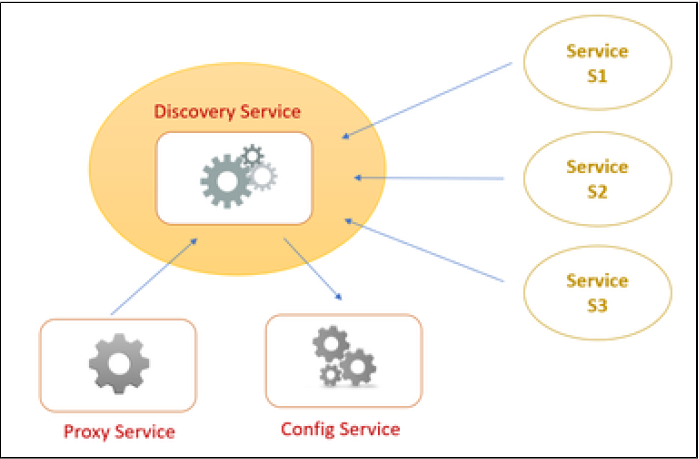
\includegraphics[width=1\columnwidth,height=0.4
\columnwidth]{images/discovery.PNG}
        \caption{Microservice Discovery-Service}
        \end{figure}
        \subsection{Structure d'un microservice}
                   \begin{figure}[H]
        \centering
        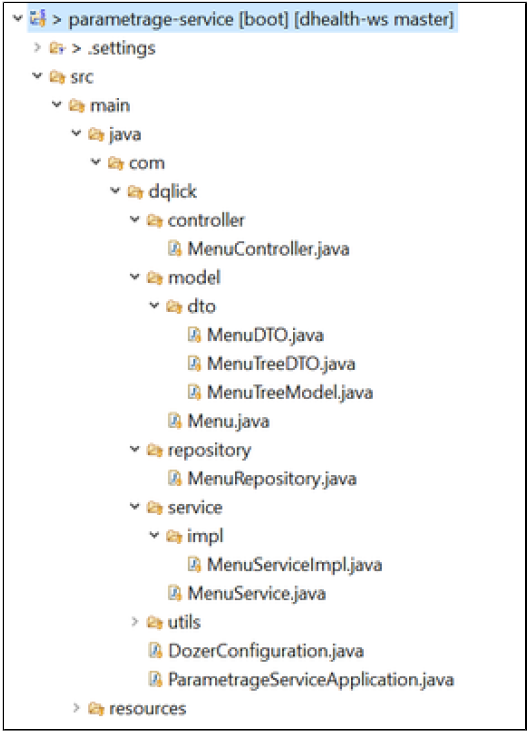
\includegraphics[width=0.8\columnwidth,height=1
\columnwidth]{images/structure.png}
        \caption{Structure d'un microservice}
        \end{figure}
    
  

\section*{Conclusion}
Dans ce chapitre, nous avons fait une étude sur les technologies que nous allons utiliser pour la réalisation de notre projet et nous avons dressé l'architecture physique de notre projet.
        \clearpage
        
        \chapter{Sprint 1: Gestion des Agences}

\section*{Introduction}
Après avoir étudié tous les aspects fonctionnels et techniques de notre projet, nous entamons la réalisation de notre projet. Pour bien appliquer la méthode Scrum que nous avons adopté. Dans ce chapitre nous détaillons l’analyse, la conception, les tests unitaires du sprint 1. Nous commençons par l’analyse fonctionnelle et la conception de ce sprint. Et à la fin, nous présentons la réalisation.

\section{Analyse}
Dans un projet Scrum, pour chaque itération on commence par la phase d’analyse et spécification du sprint. Dans cette phase on représente les diagrammes du cas d’utilisation du sprint en cours et quelques diagrammes de séquence système.

\subsection{Diagramme de cas d’utilisation raffiné}
Nous présentons ci-dessus le diagramme de cas d’utilisation raffiné qui traite la gestion des agences dans le cadre des assurances.
\newpage
Cette gestion consiste à chercher les agences par leurs compagnies et d'afficher toutes les informations qui sont:\\
-Compagnie\\
-Adresse\\
-Ville\\
-Code Postal\\
-Pays\\
-Libéllé\\

\begin{figure}[H]
\centering
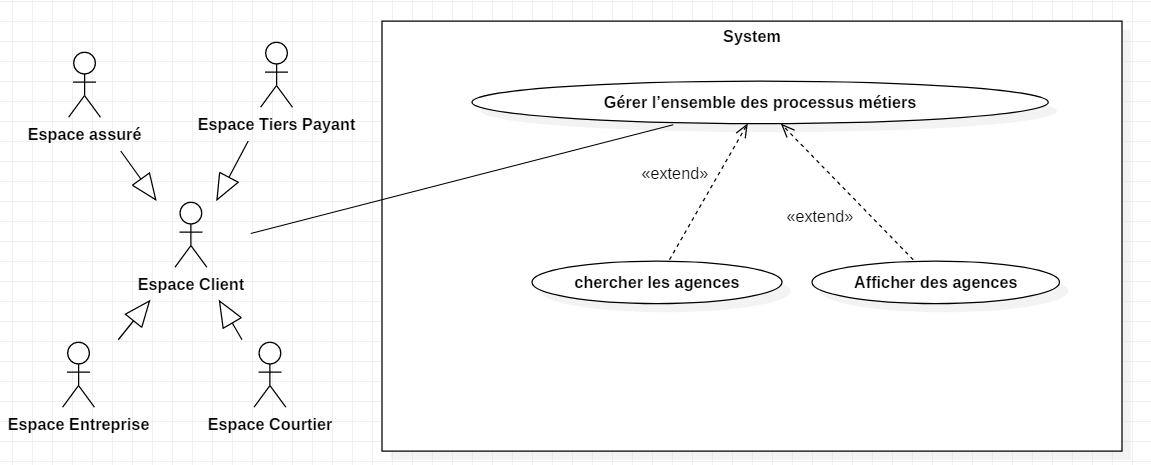
\includegraphics[width=1\columnwidth]{images/use2.PNG}
\caption{Diagramme de cas d'utilisation gestion des agences}
\label{fig:Diagramme de cas d'utilisation sprint 1}
\end{figure}

\subsection{Diagramme de séquence système}
Les diagrammes séquence système représentent l’enchaînement dynamique d’un cas d’utilisation: Gestion des agences
\begin{figure}[H]
\centering
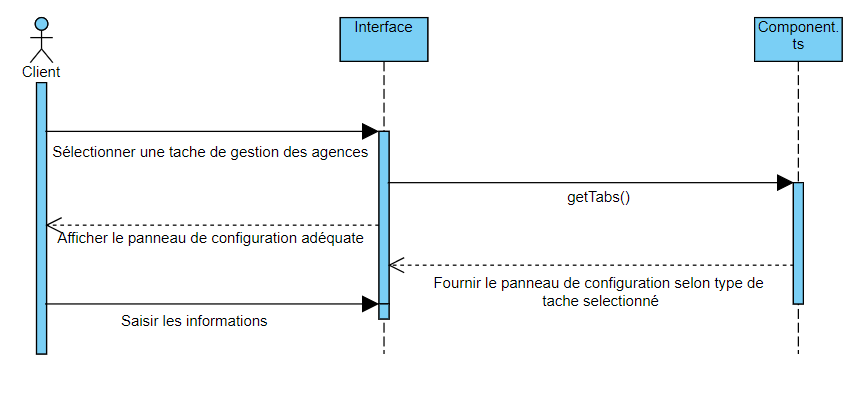
\includegraphics[width=1\columnwidth]{images/seq.PNG}
\caption{Diagramme de séquences de gestion des agences de l'assurance}
\label{fig:Diagramme de cas d'utilisation sprint 1}
\end{figure}





\section{Les tests unitaires}
Nous pouvons tester nos applications Angular de toutes pièces en écrivant et en exécutant des fonctions javascript pures. Créer des instances des classes pertinentes, appeler des fonctions et vérifier le résultat réel par rapport au résultat attendu.
En deux mots un test unitaire est un morceau de code qui valide l'unité par:\\
\textbf{L'appeler avec des intrants spécifiques.}\\
\textbf{Vérification de la sortie par rapport à la valeur attendue.}\\
Mais puisque testing est une activité si courante avec javascript, il existe un certain nombre de bibliothèques de tests et de frameworks que nous pouvons utiliser pour réduire le temps nécessaire pour écrire des tests, comme Jasmine, Mocha, QUnit et Karma.
Deux outils et frameworks de ce type qui sont utilisés lors des tests Angular sont Jasmine et Karma et qui sont les plus utilisés.
\section{IHM}
\begin{figure}[H]
\centering
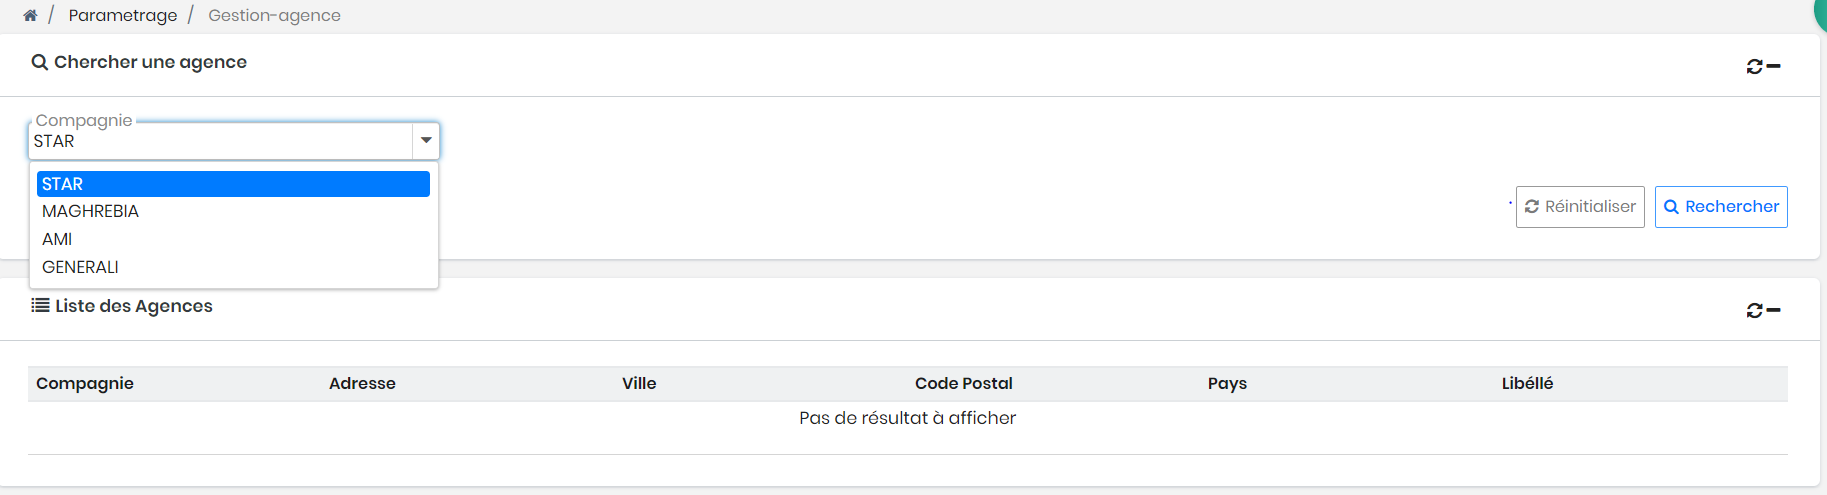
\includegraphics[width=1.05\columnwidth,height=0.45
\columnwidth]{images/interface1.PNG}
\caption{Interfaces de recherche des agences}
\label{fig:Diagramme de cas d'utilisation sprint 1}
\end{figure}





\section*{Conclusion}
Dans ce chapitre nous avons réussi à mettre en place une interface de gestions des agences. En effet, le client peut effectuer la recherche des agences en introduisant juste leur nom de compagnie.
        \clearpage
        
        \chapter{Sprint 2 : Gestion des utilisateurs }

\section*{Introduction}
Le présent chapitre détaille le deuxième module que nous avons réalisé au cours de notre projet
qui prend le cas d’utilisation "Gestion des utilisateurs". L’étude de ce sprint couvre la l’analyse, lа conception et lа réalisation.

\section{Analyse}
Dans un projet Scrum, pour chaque itération on commence par la phase d’analyse et spécification du sprint. Dans cette phase on représente le diagramme de cas d’utilisation du sprint en cours et le diagramme de séquence système.

\subsection{Diagramme de cas d’utilisation}
Nous présentons ci-dessus le diagramme de cas d’utilisation raffiné qui traite la gestion des utilisateurs des assurances.
Cette gestion consiste à chercher les utilisateurs par leurs:  noms, prénom, email, roles et d'afficher toutes les informations qui sont:\\
-Login\\
-Prénom\\
-Nom\\
-Email\\
-Rôles\\


\begin{figure}[H]
\centering
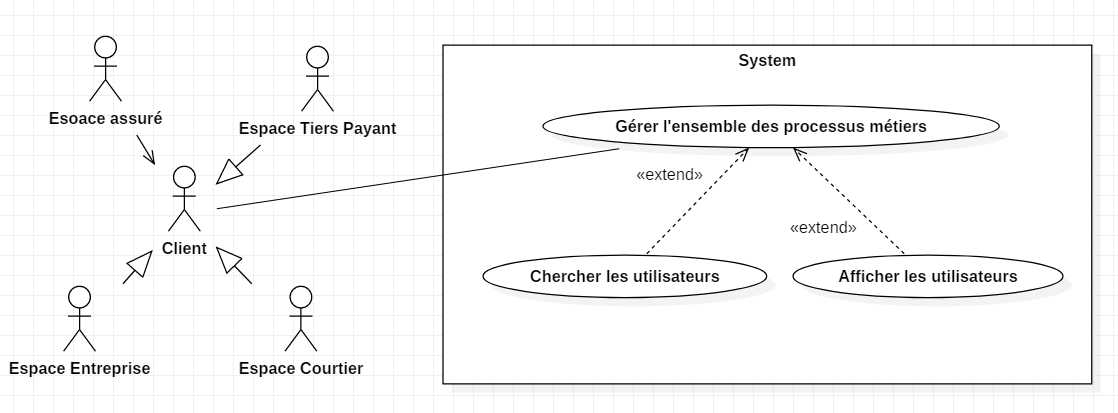
\includegraphics[width=1\columnwidth]{images/useu.PNG}
\caption{Diagramme de cas d'utilisation de gestion des utilisateurs}
\label{fig:Diagramme de cas d'utilisation sprint 1}
\end{figure}

\subsection{Diagramme de séquence système}
Les diagrammes séquence système représentent l’enchaînement dynamique d’un cas d’utilisation: Gestion des utilisateurs
\begin{figure}[H]
\centering
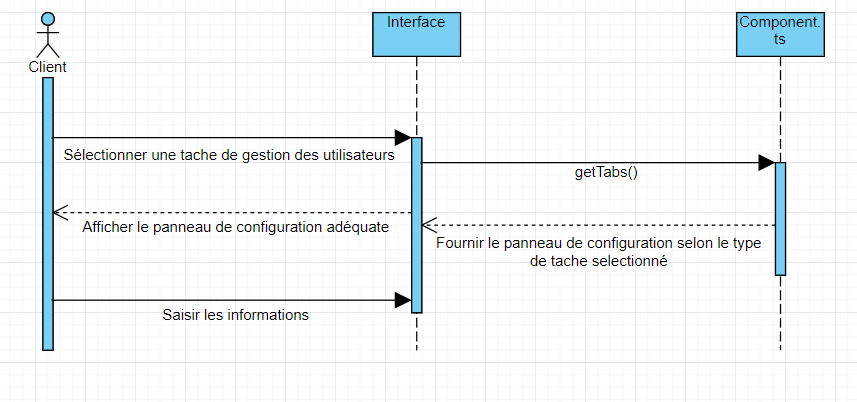
\includegraphics[width=1\columnwidth]{images/seq2.PNG}
\caption{Diagramme de séquences de gestion des utilisateurs des assurances}
\label{fig:Diagramme de cas d'utilisation sprint 1}
\end{figure}






\section{IHM}
\begin{figure}[H]
\centering
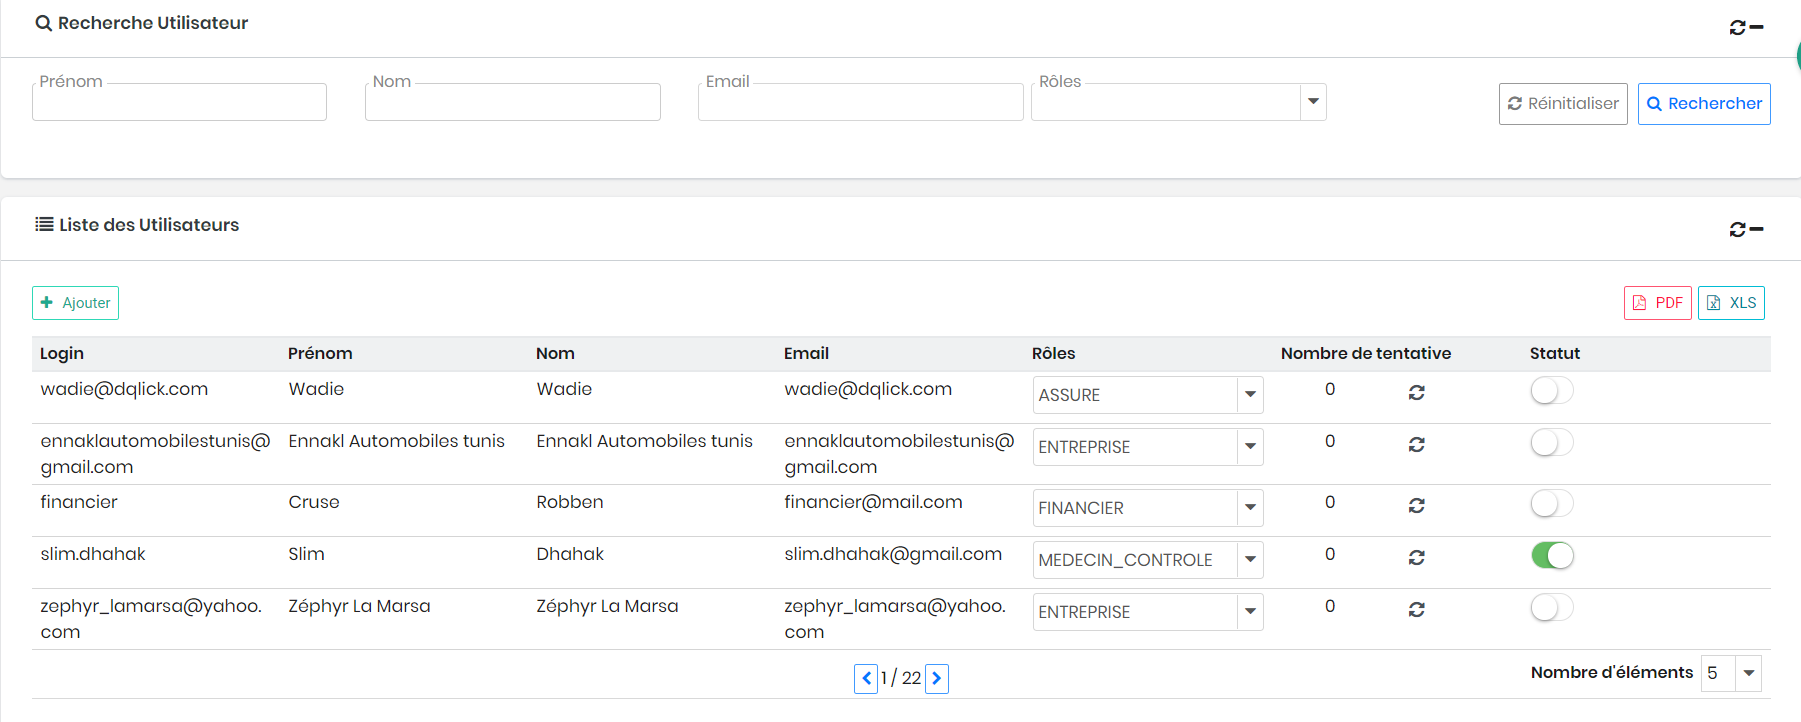
\includegraphics[width=1\columnwidth]{images/interface3.PNG}
\caption{Interface des recherches des utilisateurs}
\label{fig:Diagramme de cas d'utilisation sprint 1}
\end{figure}





\section*{Conclusion}
Dans ce chapitre nous avons réussi à mettre en place une interface de gestions des utilisateus. En effet, le client peut effectuer la recherches des utilisateurs en introduisant leurs informations personnelles et leurs roles.
       \clearpage
        
      
        \chapter*{Conclusion générale}
Ce rapport est le fruit des travaux menés au sein de l’entreprise Dqlick dans le cadre d'un stage ingénieur afin d'obtenir notre diplôme en génie Infoаrmаtique de l’ENIcarthage.

Notre travail consiste d’Implémenter deux interfaces celles des agences et des celles des utilisateurs.
Pour ce faire, nous avons commencé par présenter les concepts de base pour bien assimiler le cadre général du projet. Suite à cette étape nous avons identifié les besoins que notre application doit
satisfaire. Puis pour une bonne gestion de projet, nous avons adopté le framework Scrum car il répond à nos besoins et favorise la communication entre les différents membres de l’équipe.\\
Ce stage nous a permis de nous intégrer dans le monde professionnel, et de participer à un projet de grande envergure et à forte valeur ajoutée pour la première fois.
C’était une bonne opportunité pour mettre en œuvre nos différentes compétences acquises tout au long
de notre parcours universitaire à notre école, tout en travaillant dans une grande entreprise et au sein
d’une équipe aussi bien collaboratrice, innovante que motivante.
Malgré les changements qui ont eu lieu durant le développement, et malgré les obstacles techniques
que nous avons rencontrés, nous avons pu atteindre les objectifs que nous nous sommes fixé.


\addcontentsline{toc}{chapter}{Conclusion générale}
\markboth{Conclusion générale}{}

        \clearpage
        
        \printbibliography[heading=bibintoc]
        

    \backmatter
        %===== File containing the back cover of the document =====%
%                                                          %
%
%==========================================================%

%== It's advised to not modify the content of this file ===%
% To set your information, go to global_config.tex file    %
%==========================================================%

\thispagestyle{backcover}
\newgeometry{bottom=25mm,left=15mm,top=20mm,right=15mm}

\begin{changemargin}{3mm}{0cm}
    \begin{minipage}[c]{0.96\columnwidth}
        
       
        {\ifthenelse{\boolean{wantToTypeCompanyAddress}}
        {% IF TRUE
            \vskip5mm
        }{\vskip8mm}}
        
        \selectlanguage{frenchb}
        
        {\LARGE\textbf{Résumé}}
        \vskip1mm
            \begingroup
                \large
                \@frenchAbstract
            \endgroup
        \vskip1mm
        {\textbf{Mots clés : }
            \begingroup
                \@frenchAbstractKeywords
            \endgroup
        }
        
        {\ifthenelse{\boolean{wantToTypeCompanyAddress}}
        {% IF TRUE
            \vskip5mm
        }{\vskip8mm}}
        
        \selectlanguage{english}
        {\LARGE\textbf{Abstract}}
        \vskip1mm
            \begingroup
                \large
                \@englishAbstract
            \endgroup
        \vskip1mm
        {\textbf{Keywords : }
            \begingroup
                \@englishAbstractKeywords
            \endgroup
        }
    \end{minipage}
    
\end{changemargin}
    
\end{document}